%for JSS
%\documentclass[article]{jss}
% for vignette
\documentclass[nojss]{jss}

%%%%%%%%%%%%%%%%%%%%%%%%%%%%%%
%% declarations for jss.cls %%
%%%%%%%%%%%%%%%%%%%%%%%%%%%%%%

% Make things look better
\DefineVerbatimEnvironment{Sinput}{Verbatim}{xleftmargin=2em}
\DefineVerbatimEnvironment{Soutput}{Verbatim}{xleftmargin=2em}
\DefineVerbatimEnvironment{Scode}{Verbatim}{xleftmargin=2em}
\fvset{listparameters={\setlength{\topsep}{0pt}}}
\renewenvironment{Schunk}{\vspace{\topsep}}{\vspace{\topsep}}

% Jay's definitions
\def\btheta{\mbox{\boldmath $\theta$}}
\def\bbeta{\mbox{\boldmath $\beta$}}
\def\bgamma{\mbox{\boldmath $\gamma$}}
\def\bepsilon{\mbox{\boldmath $\epsilon$}}
\def\bmu{\mbox{\boldmath $\mu$}}
\def\bldeta{\mbox{\boldmath $\eta$}}
\def\bSigma{\mbox{\boldmath $\Sigma$}}
\def\bDelta{\mbox{\boldmath $\Delta$}}
\def\by{\textbf{y}}
\def\bA{\textbf{A}}
\def\bG{\textbf{G}}
\def\bY{\textbf{Y}}
\def\bX{\textbf{X}}
\def\bZ{\textbf{Z}}
\def\bR{\textbf{R}}
\def\bz{\textbf{z}}
\def\bW{\textbf{W}}
\def\bg{\textbf{g}}
\def\bI{\textbf{I}}
\def\var{\textrm{var}}
\def\cov{\textrm{cov}}

%% almost as usual
\author{Jay M. Ver Hoef\\NOAA, Alaska Fisheries \\Science Center \And Erin E. Peterson\\CSIRO, Division of Mathematics, \\ Informatics and Statistics \AND David Clifford\\CSIRO, Division of Mathematics, \\ Informatics and Statistics \And Rohan Shah\\ CSIRO, Division of Mathematics,\\ Informatics and Statistics}
\title{\pkg{SSN}: An \proglang{R} Package for Spatial Statistical Modeling on Stream Networks}

%% for pretty printing and a nice hypersummary also set:
\Plainauthor{Jay M. Ver Hoef, Erin E. Peterson, David Clifford, Rohan Shah} %% comma-separated
\Plaintitle{SSN: An R Package for Spatial Statistical Modeling on Stream Networks} %% without formatting
\Shorttitle{Spatial Modeling on Stream Networks} %% a short title (if necessary)

%% an abstract and keywords
\Abstract{The \pkg{SSN} package for \proglang{R} provides a set of
  functions for modeling stream network data. The package can import
  geographic information systems data or simulate new data as
  a \code{SpatialStreamNetwork}, a new object class that builds on the
  spatial \pkg{sp} classes.  Functions are provided that fit spatial
  linear models (SLMs) for the \code{SpatialStreamNetwork} object. The
  covariance matrix of the SLMs use distance metrics and
  geostatistical models that are unique to stream networks; these
  models account for the distances and topological configuration of
  stream networks, including the volume and direction of flowing
  water.  In addition, traditional models that use Euclidean distance
  and simple random effects are included, along with Poisson and
  binomial families, for a generalized linear mixed model
  framework. Plotting and diagnostic functions are provided.
  Prediction (kriging) can be performed for missing data or for a
  separate set of unobserved locations, or block prediction (block
  kriging) can be used over sets of stream segments. This article
  summarizes the \pkg{SSN} package for importing, simulating, and
  modeling of stream network data, including diagnostics and
  prediction.}

\Keywords{spatial statistics, network graphs, geostatistics,
  generalized linear mixed models}
\Plainkeywords{spatial statistics, network graphs, geostatistics,
  generalized linear mixed models}
%% without formatting
%% at least one keyword must be supplied

%% publication information
%% NOTE: Typically, this can be left commented and will be filled out by the technical editor
%% \Volume{13}
%% \Issue{9}
%% \Month{September}
%% \Year{2004}
%% \Submitdate{2004-09-29}
%% \Acceptdate{2004-09-29}

%% The address of (at least) one author should be given
%% in the following format:
\Address{
  Jay M. Ver Hoef\\
  NOAA National Marine Mammal Laboratory\\
  NMFS Alaska Fisheries Science Center\\
	International Arctic Research Center, Room 351\\
	University of Alaska Fairbanks, Fairbanks, AK  99775-7345\\
	E-mail: \email{jay.verhoef@noaa.gov}\\
	URL: \url{http://sites.google.com/site/jayverhoef} \\

  Erin E. Peterson\\
  Division of Mathematics, Informatics and Statistics\\
  Commonwealth Scientific and Industrial Research Organisation (CSIRO)\\
  PO Box 2583, Brisbane, QLD 4001\\
  E-mail: \email{Erin.Peterson@csiro.au}\\
  URL: \url{http://www.csiro.au/org/CMIS.html} \\

  David Clifford\\
  Division of Mathematics, Informatics and Statistics\\
  Commonwealth Scientific and Industrial Research Organisation (CSIRO)\\
  PO Box 2583, Brisbane, QLD 4001\\
  E-mail: \email{Erin.Peterson@csiro.au}\\
  URL: \url{http://www.csiro.au/org/CMIS.html}\\

	Rohan Shah\\
  Division of Mathematics, Informatics and Statistics\\
  Commonwealth Scientific and Industrial Research Organisation (CSIRO)\\
  PO Box 2583, Brisbane, QLD 4001\\
  E-mail: \email{Erin.Peterson@csiro.au}\\
  URL: \url{http://www.csiro.au/org/CMIS.html}
}

%% It is also possible to add a telephone and fax number
%% before the e-mail in the following format:
%% Telephone: +43/1/31336-5053
%% Fax: +43/1/31336-734

%% for those who use Sweave please include the following line (with % symbols):
%% need no \usepackage{Sweave.sty}

%% end of declarations %%%%%%%%%%%%%%%%%%%%%%%%%%%%%%%%%%%%%%%%%%%%%%%

\begin{document}





  %% include your article here, just as usual
  %% Note that you should use the \pkg{}, \proglang{} and \code{} commands.

%% Example of SWEAVE code. hide the results if this R code, do not
%% echo it in the tex document, do not save the graphics (if
%% any). Note: only one graphic can be processed from a chunk of R code.


% ------------------------------------------------------------------------------
%
%                        SECTION INTRODUCTION
%
% ------------------------------------------------------------------------------

\section{Introduction}

New spatial statistical methods were recently developed to fit models
to data collected on stream (river) networks
\citep{Ver:Pete:Move:2010}. Stream networks, in our usage, are based
on a mathematical topology that represents streams as line segments
that converge downstream, or viewed conversely, that create
dichotomous branching when moving upstream from an outlet (the most
downstream location in the network). A number of packages
\footnote{Including, but not limited to, \pkg{geoR}
\citep{Ribe:Digg:geoR:2001}, \pkg{spatial}
\citep{Vene:Ripl:mode:2002}, \pkg{geoRglm}
\citep{Chri:Ribe:geoR:2002}, \pkg{gstat} \citep{Pebe:mult:2004},
\pkg{fields} \citep{Fiel:Deve:Team:2006}, \pkg{spBayes}
\citep{Finl:Bane:Carl:spBa:2007}, and \pkg{ramps}
\citep{Smit:Yan:Cowl:unif:2008}.}  have been written in \proglang{R}
to fit spatial statistical models that use geostatistical
autocovariance functions (based on Euclidean distance), but they are
not guaranteed to produce positive-definite covariance matrices when
using an alternative distance measure, such as stream distance
\citep{Ver:Pete:Theo:spat:2006}. In this paper, we present the
\proglang{R} package \pkg{SSN}, which allows users to fit
autocovariance functions developed for stream networks
\citep{Ver:Pete:Move:2010}. These models are unique because they use
distance measured along the network, they incorporate flow direction,
and they allow covariance weighting when segments converge (e.g., by
volume of flowing water). We develop two classes of covariance models
based on moving average constructions that we call the tail-up and
tail-down models. These models may also be combined in a mixed model
strategy that includes models based on Euclidean distance. Such
geostatistical mixed models are important because they can account for
multiple processes of spatial autocorrelation in stream systems,
including those that occur within the stream and others that result
from the straight-line distances due to the terrestrial environment
\citep{Ver:Pete:Move:2010}. We note that there is another package \pkg{Rtop} for spatial prediction along stream networks \citep{Skoi:Laah:Koff:Blos:Pebe:Para:Vigl:rtop:2012}.  After describing \pkg{SSN}, we make some comparisons to \pkg{Rtop} in Section~\ref{FutureDev}. 


The \pkg{SSN} package is available on CRAN, with more information and data sets available at
\url{http://www.fs.fed.us/rm/boise/AWAE/projects/SpatialStreamNetworks.shtml}, which contains additional documentation, tutorials and example data sets. Windows and Linux binaries are provided, as well as the source code. After installation, the package is ready for use in an \proglang{R} session after typing
\begin{Schunk}
\begin{Sinput}
R> library("SSN")
\end{Sinput}
\end{Schunk}
at the \proglang{R} prompt.  To ensure that you have full read and write permissions, and that you do not leave stray files on your computer, use the following
\begin{Schunk}
\begin{Sinput}
R> file.copy(system.file("lsndata/MiddleFork04.ssn", package = "SSN"),
+    to = tempdir(), recursive = TRUE, copy.mode = FALSE)
\end{Sinput}
\begin{Soutput}
[1] TRUE
\end{Soutput}
\begin{Sinput}
R> setwd(tempdir())
\end{Sinput}
\end{Schunk}

The rest of the paper is organized as follows:
Section~\ref{TheoryModels} provides a brief overview of spatial
statistical modelling on stream networks. Section~\ref{S4SSNobject}
provides an overview of the \code{S4} \code{SpatialStreamNetwork}
object, while Section~\ref{manipSSNobj} describes how to set up and
manipulate the object. Section~\ref{dataAnaSSN} describes the main
statistical capabilities provided by the package, including
exploratory data analysis, model fitting, model evaluation and
diagnostics, as well as prediction. Section~\ref{Simulation} shows how
to simulate stream network data. Finally, Section~\ref{FutureDev}
provides a brief discussion of future developments.

This document was compiled on 2014-01-20 using
R version 3.0.2 (2013-09-25).

% ------------------------------------------------------------------------------
%
% SPATIAL STATISTICAL MODELS FOR STREAM NETWORKS
%
% ------------------------------------------------------------------------------

\section{Spatial statistical models on stream networks} \label{TheoryModels}

Some new models for stream networks, based on moving average
constructions, were initially described by
\citet{Ver:Pete:Theo:spat:2006} and
\citet{Cres:Frey:Harc:Smit:spat:2006}. The models used stream
distance measures \citep*[e.g.,][]{Dent:Grim:spat:1999}, where stream
distance is defined as the shortest distance between two locations
computed only along the stream network. This work was summarized by
\citet{Ver:Pete:Move:2010}, which provides more technical
details. Here, we give a brief summary.

% -------------------Notation

\subsection{Background}

The fact that streams are dichotomous and have flow creates a rich set
of models not seen in either time-series or spatial statistics.  The
models are created using moving average constructions.  If a moving
average function starts at some location and is non-zero only upstream
of that location, we call them ``tail-up'' models. Due to the
dichotomous nature of streams, the moving average function may need to
split as it goes upstream in order to produce stationary models, so
some weighting must occur. If a moving average function starts at some
location and is non-zero only downstream of that location, we call
them ``tail-down'' models. A full development of these models is given
in \citet{Ver:Pete:Move:2010}. Consider two pairs of sites that have
the same stream distance between them, but one pair is connected by
flowing water (i.e., flow-connected), and the other pair is not
connected by flowing water (i.e., flow-unconnected); in general the
amount of autocorrelation will be different between them. For the
following development, let $r_i$ and $s_j$ denote two locations on a
stream network, and let $h$ be the stream distance between them.  Then
the following covariance models have been developed and implemented in
the \pkg{SSN} package.

% -------------------Tail-up Models

\subsection{Tail-up models}\label{tailup}

The moving average construction as described by \citet{Ver:Pete:Theo:spat:2006} is
%
% COVARIANCE DERIVED FROM MOVING AVERAGE DEFINITION
%
\begin{equation} \label{eq:moveaveup} C_u(r_i,s_j|\btheta_u)=
  \left\{ \begin{array}{ll} \pi_{i,j}C_t(h|\btheta_u) &
      \textrm{if $r_i$ and $s_j$ are flow-connected,} \\
      0 & \textrm{if $r_i$ and $s_j$ are flow-unconnected,}
	\end{array} \right.
\end{equation}
%
where $\pi_{i,j}$ are weights due to branching characteristics of the
stream, and the function $C_t(h|\btheta_u)$ can take the following
forms:

\begin{itemize}
\item Tail-up Linear-with-Sill Model,
  \[
  C_t(h|\btheta_u)=
  \sigma^2_u\left(1 -\frac{h}{\alpha_u}\right)I\left(\frac{h}{\alpha_u}\leq 1\right),
  \]
\item Tail-up Spherical Model,
  \[
  C_t(h|\btheta_u)=
  \sigma^2_u\left(1-\frac{3}{2}\frac{h}{\alpha_u}+\frac{1}{2}\frac{h^3}{\alpha_u^3}\right)
  I\left(\frac{h}{\alpha_u}\leq 1\right),
  \]
\item Tail-Up Exponential Model,
  \[
  C_t(h|\btheta_u)= \sigma^2_u\exp(-3h/\alpha_u),
  \]
\item Tail-up Mariah Model,
  \[
  C_t(h|\btheta_u)= \left\{ \begin{array}{ll}
      \sigma^2_u\left(\frac{\log(90h/\alpha_u+1)}{90h/\alpha_u}\right) &
      \textrm{if} \; h > 0,\\
      \sigma^2_u &
      \textrm{if} \; h = 0,\\
    \end{array} \right.
  \]
\item Tail-up Epanechnikov Model \citep{Garr:Mone:Ver:spat:2009},
  \[
  C_t(h|\btheta_u)=
      \frac{\sigma^2_u(h-\alpha_u)^2f_{eu}(h;\alpha_u)}{16\alpha_u^5} 
	I\left(\frac{h}{\alpha_u}\leq 1\right).
	\]
\end{itemize}
where $f_{eu}(h;\alpha_u)=16\alpha_u^2 + 17\alpha_u^2h - 2\alpha_uh^2-h^3$, $I(\cdot)$ is the indicator function (equal to one when the
argument is true), $\sigma^2_u > 0$ is an overall variance parameter
(also known as the partial sill), $\alpha_u > 0$ is the range
parameter, and $\btheta_u = (\sigma^2_u,\alpha_u)^\top$. Note the
factors 3, and 90 for the exponential and mariah models, respectively,
which cause the autocorrelation to be approximately 0.05 when $h$
equals the range parameter.  This helps compare range parameters
($\alpha_u$) across models. (The distance at which autocorrelation
reaches 0.05 is sometimes called the effective range when models
approach zero asymptotically.)

\subsection{Weights for tail-up models}\label{tailupWeights}

For the weights, $\pi_{i,j}$, consider the following example.  First
associate a weight of 1 with each source (upper-most) segment in a
stream network. When two segments converge at a junction the weight
for the segment downstream of the junction is the sum of the two
upstream weights, creating an additive function when moving
downstream. Segment weights formed in this manner are known as
Shreve's stream order \citep{Shre:infi:1967}. These additive weights
are a property of whole stream segments, creating a step function
along a stream network. Any point on a stream network has an additive
function value obtained from the stream segment where it occurs. If we
denote the value of the additive function as $\Omega(x)$ for some
point $x$ on the stream network, then for two flow-connected points
where $r_i$ is downstream from $s_j$,
\[ \pi_{i,j}=\sqrt{\frac{\Omega(s_j)}{\Omega(r_i)}}.  \]

More details can be found in \citet{Ver:Pete:Move:2010}, including
ways to create an additive function from arbitrary values associated
with stream segments, such as flow volume or a proxy for flow volume
(e.g., basin area).

% -------------------Tail-down Models

\subsection{Tail-down models}\label{taildown}

For tail-down models, we distinguish between the flow-connected and
flow-unconnected situation.  When two sites are flow-unconnected, let
$b$ denote the longer of the distances to the common downstream
junction, and $a$ denote the shorter of the two distances.  If two
sites are flow-connected, again use $h$ to denote their separation
distance via the stream network. The following are tail-down models:

\begin{itemize}
\item Tail-Down Linear-with-Sill Model, $b \geq a \geq 0$,
  \[
  C_d(a,b,h|\btheta_d)= \left\{ \begin{array}{ll}
      \sigma^2_d\left(1 -\frac{h}{\alpha_d}\right)I\left(\frac{h}{\alpha_d}\leq 1\right) &
      \textrm{if flow-connected,}\\
      \sigma^2_d\left(1 -\frac{b}{\alpha_d}\right)I\left(\frac{b}{\alpha_d}\leq 1\right) &
      \textrm{if flow-unconnected,}
    \end{array} \right.
  \]
\item Tail-Down Spherical Model, $b \geq a \geq 0$,
  \[
  C_d(a,b,h|\btheta_d)= \left\{ \begin{array}{ll}
      \sigma^2_d(1-\frac{3}{2}\frac{h}{\alpha_d}+\frac{1}{2}\frac{h^3}{\alpha_d^3})I\left(\frac{h}{\alpha_d}\leq 1\right) &
      \textrm{if flow-connected,}\\
      \sigma^2_d\left(1-\frac{3}{2}\frac{a}{\alpha_d}+\frac{1}{2}\frac{b}{\alpha_d}\right)
      \left(1- \frac{b}{\alpha_d}\right)^2I\left(\frac{b}{\alpha_d}\leq 1\right) &
      \textrm{if flow-unconnected,}
    \end{array} \right.
  \]
\item Tail-down Exponential Model,
  \[
  C_d(a,b,h|\btheta_d)= \left\{ \begin{array}{ll}
      \sigma^2_d\exp(-3h/\alpha_d) &
      \textrm{if flow-connected,}\\
      \sigma^2_d\exp(-3(a+b)/\alpha_d) &
      \textrm{if flow-unconnected,}
    \end{array} \right.
  \]
\item Tail-down Mariah Model,
  \[
  C_d(a,b,h|\btheta_d)= \left\{ \begin{array}{ll}
      \sigma^2_d\left(\frac{\log(90h/\alpha_d+1)}{90h/\alpha_d}\right) &
      \textrm{if flow-connected, } h > 0,\\
      \sigma^2_d	& \textrm{if flow-connected, } h = 0,\\
      \sigma^2_d\left(\frac{\log(90a/\alpha_d+1)-\log(90b/\alpha_d+1)}{90(a-b)/\alpha_d}\right) &
      \textrm{if flow-unconnected, } a \ne b, \\
      \sigma^2_d\left(\frac{1}{90a/\alpha_d+1}\right) &
      \textrm{if flow-unconnected, } a = b,
    \end{array} \right.
  \]
\item Tail-down Epanechnikov Model, $b \geq a \geq 0$,
  \[
  C_d(a,b,h|\btheta_d)= \left\{ \begin{array}{ll}
      \frac{\sigma^2_d(h-\alpha_d)^2f_{eu}(h;\alpha_d)}{16\alpha_d^5} 
	I\left(\frac{h}{\alpha_u}\leq 1\right) &
      \textrm{if flow-connected,}\\
      \frac{\sigma^2_d(b-\alpha_d)^2f_{ed}(a,b;\alpha_d)}{16\alpha_d^5} 
	I\left(\frac{b}{\alpha_u}\leq 1\right) &
      \textrm{if flow-unconnected,}
    \end{array} \right.
  \]
\end{itemize}
where $f_{ed}(a,b;\alpha_d)=16\alpha_d^3 + 17\alpha_d^2b - 15\alpha_d^2a - 20\alpha_da^2 - 2\alpha_db^2 + 10\alpha_dab + 5ab^2 - b^3 - 10ba^2$, $\sigma^2_d > 0$ and $\alpha_d > 0$, and $\btheta_d = (\sigma^2_d,\alpha_d)^\top$.  Although not necessary to maintain stationarity, the weights used in the tail-up models can be applied to the tail-down models as well.  Note that $h$ is unconstrained, because for model-building we imagine that the headwater and outlet segments continue to infinitiy, as first described by \citet{Ver:Pete:Theo:spat:2006}. Also note that $a$ does not appear in the tail-down linear-with-sill model, but is used indirectly because the model depends on the point that is farthest from the junction; i.e., $b$, and so $a$ is the shorter of the two distances.

% -------------------Euclidean Distance Models

\subsection{Euclidean distance models}\label{EucDist}

The 2-D coordinate system is used to include Euclidean distance
models, which are described in many textbooks
\citep*[e.g.,][]{Cres:stat:1993,Chil:Delf:geos:1999}.  We include four
models and show their parameterization in the \pkg{SSN} package.  If
site $r_i$ has x,y-coordinates $(x_i,y_i)$ and site $s_j$ has
x,y-coordinates $(x_j,y_j)$, then the Euclidean distance is defined as
$d=\sqrt{(x_i-x_j)^2+(y_i-y_j)^2}$, and we have the following models:

\begin{itemize}
\item Euclidean Distance Cauchy Model,
  \[
  C_e(d|\btheta_e)=
  \sigma^2_e\left(1 + 4.4(d/\alpha_e)^2\right)^{-1},
  \]
\item Euclidean Distance Spherical Model,
  \[
  C_e(d|\btheta_e)=
  \sigma^2_e\left(1-\frac{3}{2}\frac{d}{\alpha_e}+\frac{1}{2}\frac{d^3}{\alpha_e^3}
  \right)I\left(\frac{d}{\alpha_e}\leq 1\right),
  \]
\item Euclidean Distance Exponential Model,
  \[
  C_e(d|\btheta_e)=
  \sigma^2_e\exp(-3d/\alpha_e),
  \]
\item Euclidean Distance Gaussian Model,
  \[
  C_e(d|\btheta_e)=
  \sigma^2_e\exp(-3(d/\alpha_e)^2).
  \]
\end{itemize}
Note the factors 3, 3, and 4.4 for the exponential, Gaussian, and
Cauchy models, respectively, which cause the autocorrelation to be
approximately 0.05 when $d$ equals the range parameter.

\subsection{Random effects models}

The \pkg{SSN} package provides the functionality to fit random effect
models associated with factor variables. Let $\gamma_k(x)$ denote the
factor level at location $x$. Each level of $\gamma_k$ is assumed to
be a random quantity with mean 0 and variance $\sigma^2_k$ and these
are independently and identically distributed. As such, sites with the
same level of $\gamma_k$ are correlated, and sites with different
levels of $\gamma_k$ are uncorrelated,

\begin{equation}
  C_{k}(r_i,s_j)= \left\{ \begin{array}{ll}
      \sigma_i^2 &
      \textrm{if $\gamma_k(r_i) = \gamma_k(s_j)$}, \\
      0 &
      \textrm{if $\gamma_k(r_i) \neq \gamma_k(s_j).$ }
    \end{array} \right.
\end{equation}

% -------------------Mixed Models

\subsection{Spatial linear mixed models} \label{sec:SpatialLinearMixedModels}

The most general linear model that the \pkg{SSN} package considers is
\begin{equation} \label{eq:spLinearModel}
\bY = \bX\bbeta + \bz_u + \bz_d +\bz_e + \bW_1\bgamma_1 + \ldots
+ \bW_p\bgamma_p + \bepsilon,
\end{equation}
where $\bX$ is a design matrix of fixed effects, $\bbeta$ are
parameters, the vector $\bz_u$ contains spatially-autocorrelated
random variables with a tail-up autocovariance, with $\var(\bz_u) =
\sigma_u^2\bR(\alpha_u)$ and $\bR(\alpha_u)$ is a correlation matrix
that depends on the range parameter $\alpha_u$ as described in
Section~\ref{tailup}; $\bz_d$ contains spatially-autocorrelated random
variables with a tail-down autocovariance, $\var(\bz_d) =
\sigma_d^2\bR(\alpha_d)$ as described in Section~\ref{taildown};
$\bz_e$ contains spatially-autocorrelated random variables with a
Euclidean distance autocovariance, $\var(\bz_e) =
\sigma_e^2\bR(\alpha_e)$ as described in Section~\ref{EucDist};
$\bW_k$ is a design matrix for random effects $\bgamma_k; k =
1,\ldots,p$ with $\var(\bgamma_k)=\sigma^2_k\bI$, and $\bepsilon$
contains independent random variables with
$\var(\bepsilon)=\sigma^2_0\bI$.  When used for spatial prediction,
this model is referred to as ``universal'' kriging
\citep*[p. 107]{Le:Zide:stat:2006} , with ``ordinary'' kriging being
the special case where the design matrix \textbf{X} is a single column
of ones \citep[p. 119]{Cres:stat:1993}. The most general covariance
matrix considered by the \pkg{SSN} package is of the form
\begin{equation} \label{eq:covStructure}
\cov(\bY)=\bSigma=\sigma_u^2\bR(\alpha_u) + \sigma_d^2\bR(\alpha_d) +
\sigma_e^2\bR(\alpha_e) + \sigma_1^2\bW_1\bW_1^\top + \ldots +
\sigma_p^2\bW_p\bW_p^\top + \sigma_0^2\bI.  \end{equation} The
\pkg{SSN} package uses either maximum likelihood (ML) or restricted
maximum likelihood (REML) to estimate $\bbeta$ and some subset of the
possible covariance parameters \\
$\btheta=(\btheta_u^\top,\btheta_d^\top, \btheta_e^\top, \sigma^2_1,
\ldots, \sigma^2_p, \sigma^2_0)^\top$, as specified by the user.

% ---------------Generalized Linear Models using Pseudo-data

\subsection{Spatial generalized linear mixed models}\label{SpGenLinMixMod}

The \pkg{SSN} package estimates parameters for generalized linear
mixed models using pseudo-models as described by
\citet{Wolf:Ocon:gene:1993}. For time series and other spatial
covariance structures, pseudo-models are implemented in the
\code{glmmPQL} function in the \pkg{MASS} package
\citep{Vene:Ripl:mode:2002}.  At present, only binomial and Poisson
distributions are supported in the \pkg{SSN} package. Consider the
expectation of the response variable as a linear mixed model through a
link function,
%
% Generalized linear model mean specification
%
\begin{equation} \label{glm.mean}
	 E(\bY|\bgamma) =
	   g^{-1}(\bX \bbeta + \bW \bgamma) =
	   g^{-1}(\bldeta) = \bmu,
\end{equation}
%
where $g$ is the link function. Suppose that we have a current
estimates of $\bbeta$ and $\bgamma$; call them $\tilde{\bbeta}$ and
$\tilde{\bgamma}$. Initial estimates could be obtained using the
\code{glm()} function, which assumes independence among data.  Then
pseudo-data are formed as
%
% Pseudo data
%
\begin{equation} \label{pseudo.data}
	\tilde{\bY} \equiv \tilde{\bDelta}^{-1}(\bY -
	  g^{-1}(\bX \tilde{\bbeta} + \bW \tilde{\bgamma})) +
	  \bX \tilde{\bbeta} + \bW \tilde{\bgamma},
\end{equation}
where
\[
   \tilde{\bDelta} \equiv
     \frac{\partial g^{-1}(\bldeta)}
     {\partial \bldeta}
\]
is a diagonal matrix evaluated at $\tilde{\bbeta}$ and $\tilde{\bgamma}$.
Then the pseudo-model is
%
% Pseudo model
%
\begin{equation} \label{pseudo.model}
	 \tilde{\bY} = \bX\bbeta + \bW\bgamma + \bepsilon.
\end{equation}
Note that the left-hand side of Equation~\ref{pseudo.model} depends on
$\tilde{\bbeta}$ and $\tilde{\bgamma}$, so that suggests an iterative
procedure for updating $\bbeta$ and $\bgamma$.  The covariance matrix
specification of pseudo-data is assumed to be
\[
   \textrm{var}(\bepsilon) =
     \tilde{\bDelta}^{-1}\bA^{\frac{1}{2}}\sigma^2\bR
       \bA^{\frac{1}{2}}\tilde{\bDelta}^{-1},
\]
where $\bA$ is a diagonal matrix and contains the variance functions
of the model \citep*[e.g.,][Table 2.1]{McCu:Neld:gene:1989}. The
matrix $\bR$ is a correlation matrix as in
Equation~\ref{eq:covStructure}.  The most general covariance matrix of
the linear mixed pseudo-model considered by the \pkg{SSN} package is
%
% marginal covariance matrix of linear mixed pseudo-model
%
\begin{equation} \label{eq:pseudo.marg.cov}
	\begin{array}{c}
  \cov(\tilde{\bY}) = \tilde{\bDelta}^{-1}\bA^{\frac{1}{2}}
	[\sigma_u^2\bR(\alpha_u) + \sigma_d^2\bR(\alpha_d) +
	\sigma_e^2\bR(\alpha_e) + \sigma_0^2\bI]
	\bA^{\frac{1}{2}}\tilde{\bDelta}^{-1} + \\
	\sigma_1^2\bW_1\bW_1^\top + \ldots +
	\sigma_p^2\bW_p\bW_p^\top.
	\end{array}
\end{equation}
The iterative algorithm of \citet{Wolf:Ocon:gene:1993} is implemented
as the following steps: 1) the parameters $\tilde{\bbeta}$ and
$\tilde{\bgamma}$ and pseudo-data $\tilde{\bY}$ are updated using an
iteratively weighted least squares algorithm
\citep[e.g.,][pg. 40]{McCu:Neld:gene:1989} for a fixed covariance
model (Equation~\ref{eq:pseudo.marg.cov}), and then 2) the covariance
parameters $\btheta$ of Equation~\ref{eq:pseudo.marg.cov} are updated
using ML or REML for fixed $\tilde{\bY}$.

% ------------------------------------------------------------------------------
%
%            THE S4 SpatialStreamNetwork OBJECT
%
% ------------------------------------------------------------------------------

\section[The S4 SpatialStreamNetwork object]{The \code{S4} \code{SpatialStreamNetwork} object} \label{S4SSNobject}

\subsection{Input data}

The spatial data needed to fit a stream network model are
non-trivial. Much of the spatial data editing, information generation,
and formatting take place in ArcGIS version 9.3.1 using the Spatial
Tools for the Analysis of River Systems (\pkg{STARS}) toolset
(Peterson and Ver Hoef in review). When this pre-processing is
complete, a new directory is created to store the data, hereafter
referred to as the \code{.ssn} directory, which can then be imported
into \proglang{R}. These data include the feature geometry, attribute
data, and topological relationships of each point and line data set,
see Figure~\ref{dotSSNdirectory}.

\begin{figure}[htbp]
  \begin{center}
    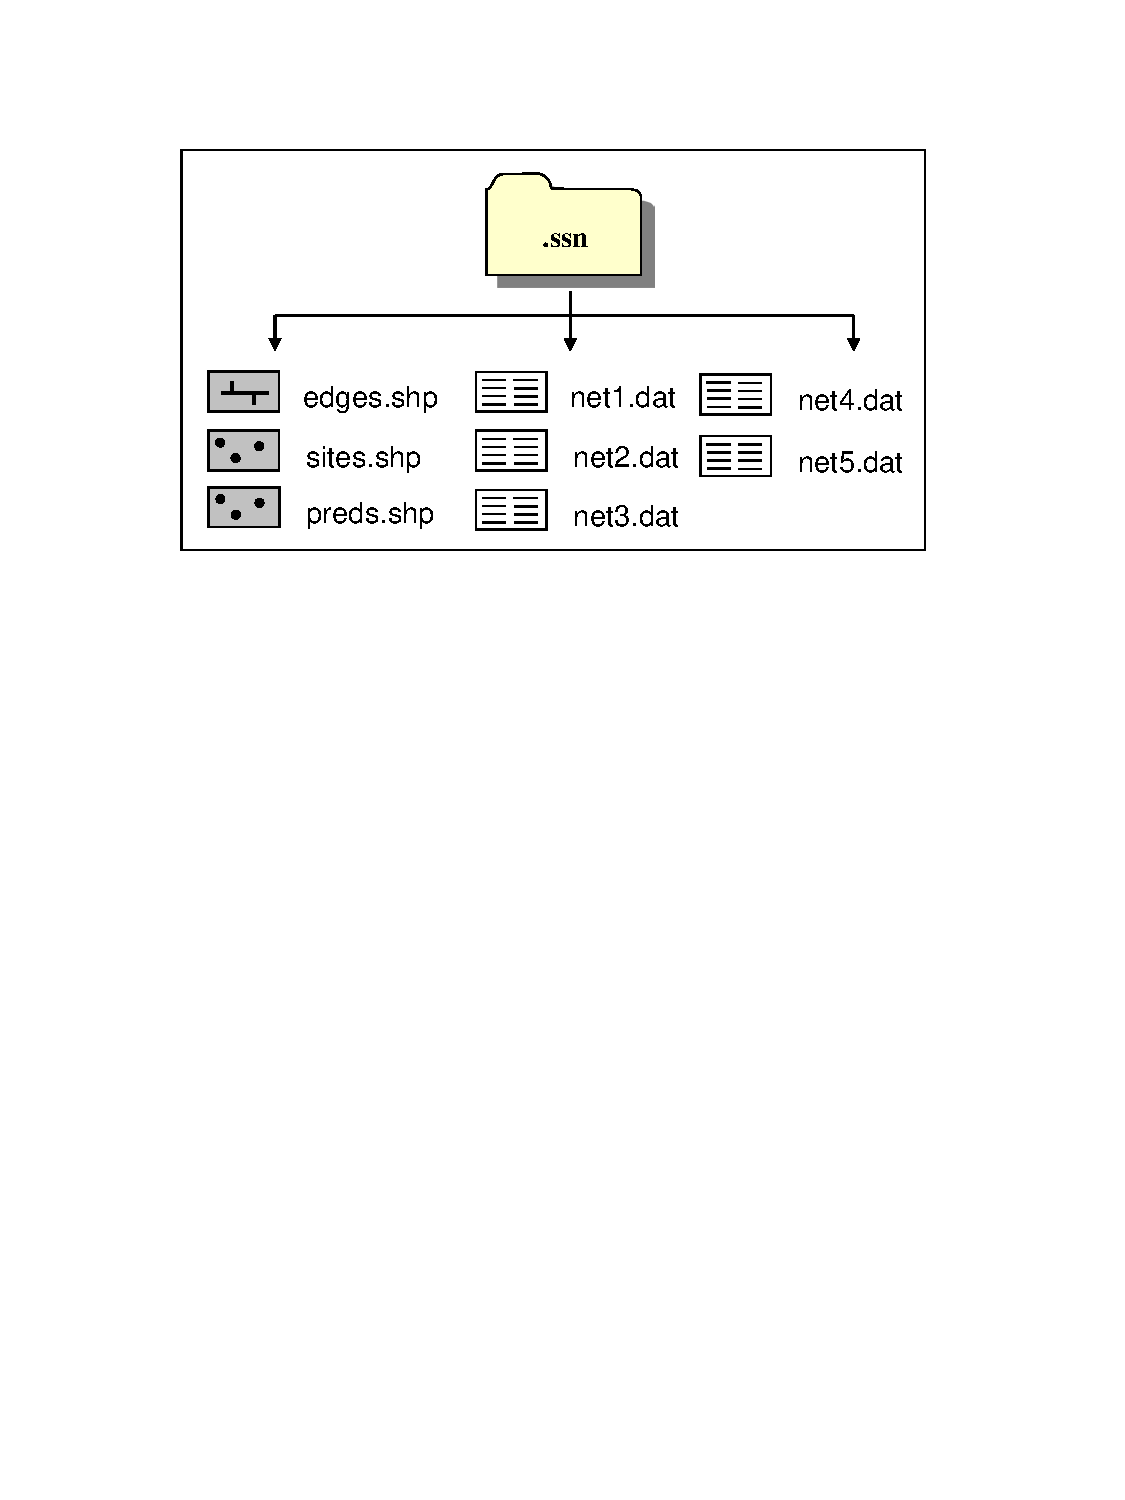
\includegraphics[height=250pt,keepaspectratio]{Figures/jss984Fig-dotSSNdirectory.pdf}
  \end{center}
  \caption{The \code{.ssn} directory contains the spatial, attribute, and
    topological information needed to create a \code{SpatialStreamNetwork}
    object in \proglang{R}. The *.shp files are of stream reaches (edges.shp), observed points on the stream (site.shp), and prediction points on the stream (preds.shp)(optional). The *.dat files contain topological relationship information for each distinct network; in this example, there are 5 networks. \label{dotSSNdirectory}}
\end{figure}

The \code{.ssn} directory will always contain two shapefiles: edges
and sites, which contain the geometry and attribute information for
the stream network and the observed data locations. Multiple
comma-delimited text files containing the topological information for
each stream network within the edges data set will also be
included. Here, a network is defined as a set of connected, directed
line segments that share a common junction somewhere downstream. Note
that the naming conventions for these files are implemented by the
\pkg{STARS} toolset and must be preserved. Multiple shapefiles
representing the prediction locations may also be included in the
\code{.ssn} directory; however, the naming conventions for these data
sets will vary. Please see Peterson and Ver Hoef (in review) for a
detailed description of the \pkg{STARS} toolset, the methods used to
generate the .ssn directory, and data therein.

\subsection{Object structure}

The \code{SpatialStreamNetwork} class is an \code{S4} object
(Figure~\ref{SSNclass}), which is the foundational spatial data class
in the \pkg{SSN} package. Its structure adheres to the conventions for
spatial data classes set out by
\citet{Biva:Pebe:Gome:appl:2008}. Yet, the
\code{SpatialStreamNetwork} is unique because it contains both point
and line features within the same \code{S4} object. It directly
extends class \code{SpatialLinesDataFrame}, with additional slots
included to store the spatial point data \code{SSNPoints}, a matrix
containing information about the network coordinates of each line
segment \code{network.line.coords}, as well as a string representing
the filepath to the \code{.ssn} directory. A new class,
\code{SSNPoint}, has been defined and created to store spatial point
data for observation and prediction locations. This class is similar
to class \code{SpatialPointsDataFrame}, but is not a direct extension
of it since common slot names contain the prefix ``point.'' An
additional matrix containing network coordinates,
\code{network.point.coords}, has also been included. The object
\code{SSNPoints} is a list of class \code{SSNPoints} that stores
objects of class \code{SSNPoint}. It also contains a slot named
\code{ID}, which holds a string identifier for each \code{SSNPoint}
object.This allows identification within the
\code{SpatialStreamNetwork} object when multiple data sets of
prediction sites are included.

The purpose of the \code{.ssn} directory is to store information about
spatial relationships generated in \proglang{R}, in addition to
holding the input data. When the \code{SpatialStreamNetwork} class is
created, the topological information contained in text files is
imported into a SQLite database using the \pkg{RSQLite} package
\citep{Jame:appl:2011}. This database is named \code{binaryID.db} and
contains a separate table for each network, which holds the
topological information of the network, including reach identifiers
(\code{rid}) and binary identifiers (\code{ID}). The \code{rid}s are
unique to each line segment in the entire edges data set, while binary
\code{ID}s are unique to each line segment within a network, see
Figure~\ref{SSNclass}.

\begin{figure}[ht]
  \begin{center}
      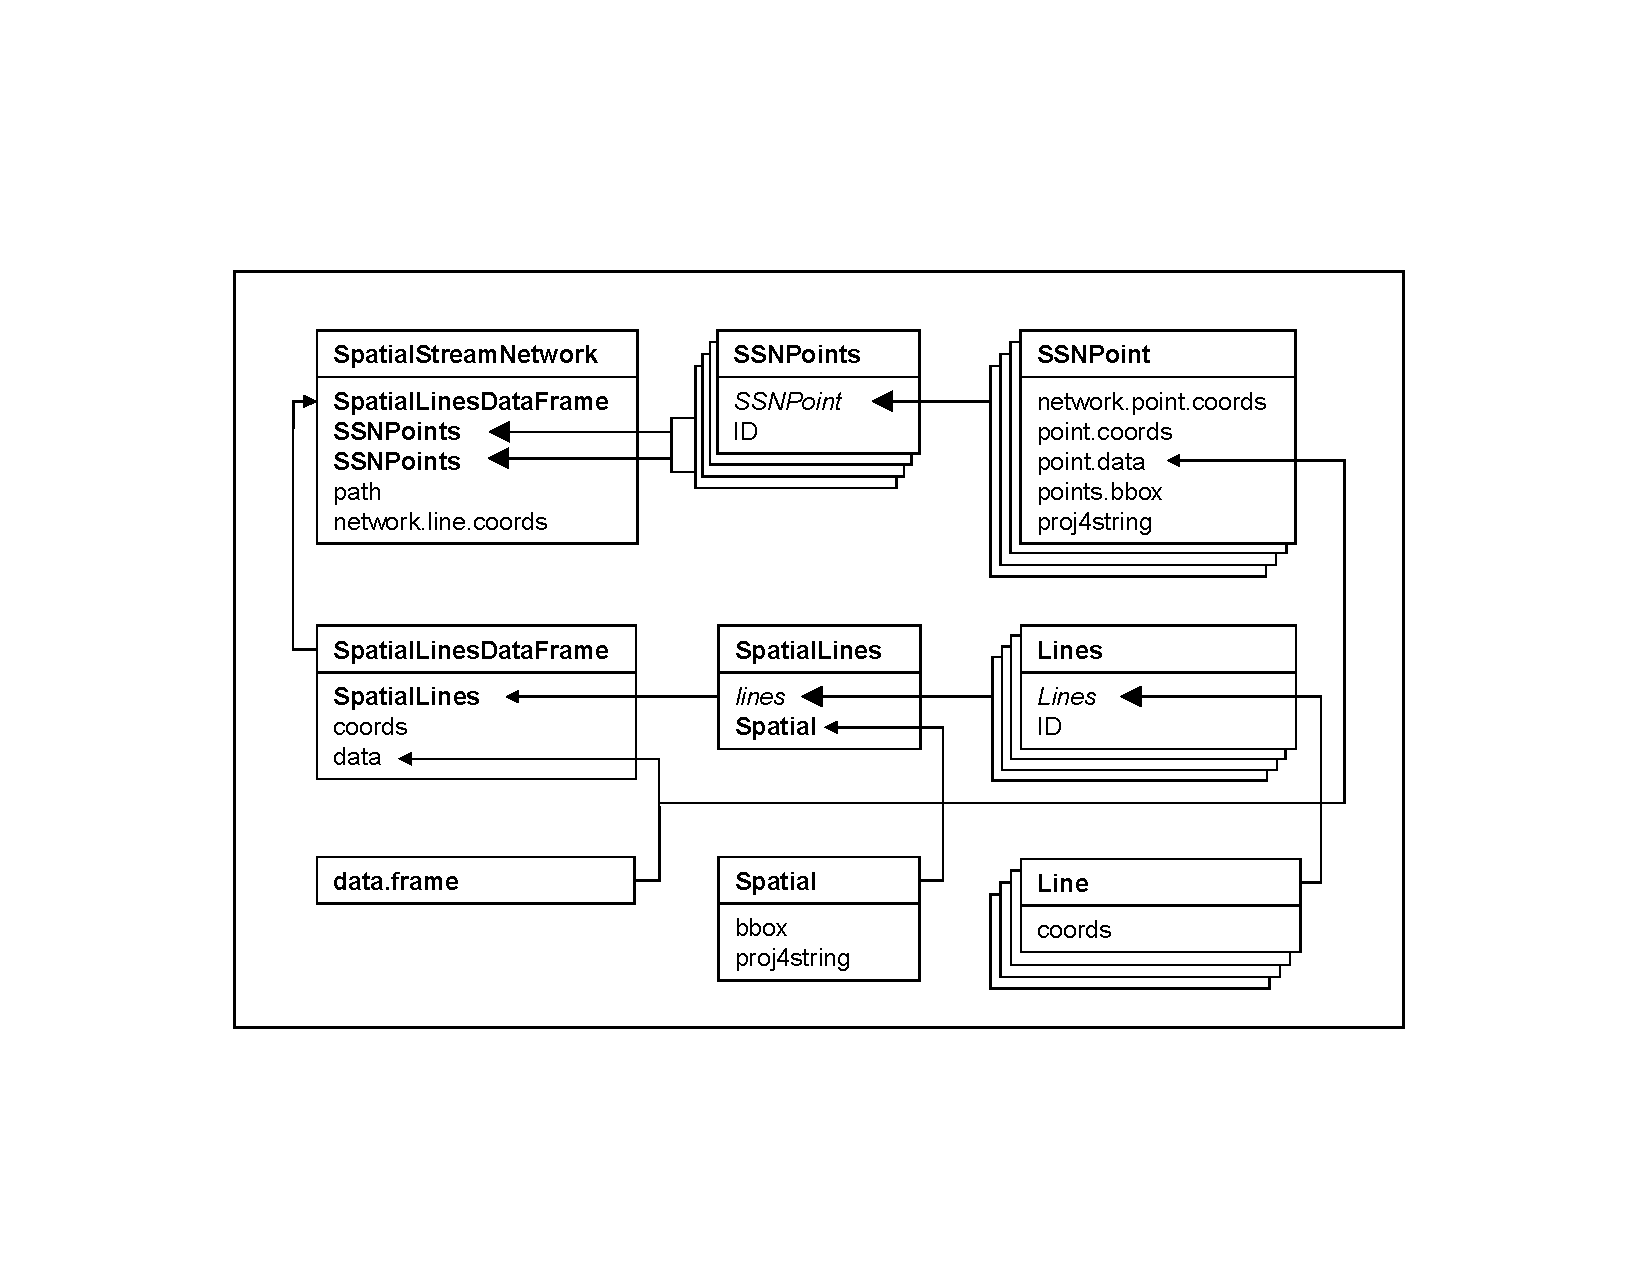
\includegraphics[width=\textwidth,keepaspectratio]{Figures/jss984Fig-SSNclass.pdf}
  \end{center}
  \caption{The \code{SpatialStreamNetwork} class and slots; arrows with small heads show
    sub-class extensions and arrows with large heads show the inclusion of lists of
    objects. \label{SSNclass}}
\end{figure}

Peterson and Ver Hoef (in review) give additional details about
the binary IDs and how they are used to assess spatial relationships
within a network.


% ------------------------------------------------------------------------------
%
%            MANIPULATING THE SpatialStreamNetwork OBJECT
%
% ------------------------------------------------------------------------------

\section[Manipulating the SpatialStreamNetwork object]{Manipulating the \code{SpatialStreamNetwork} object}\label{manipSSNobj}

The \pkg{SSN} package provides functions to import and export
\code{SpatialStreamNetwork} objects. These objects may be created
using the \pkg{STARS} ArcGIS custom toolbox for version 9.3.1
(Peterson and Ver Hoef in review).  It is also possible to simulate a
\code{SpatialStreamNetwork} with both observed and prediction
locations in \proglang{R}. Regardless of the way the object is
generated, it contains important spatial information about feature
geometry, attribute data, and topological relationships. These
relationships must be represented in \proglang{R} to create the
spatial information needed to fit a spatial statistical model. These
capabilities are further explored below.

\subsection[Data available in the SSN package]{Data available in the \pkg{SSN} package}

A data set is included in the \pkg{SSN} package as well as code to
simulate data on simulated stream networks. The data set is from the Middle Fork, a stream in Idaho, United States, and is a subset of a larger data set than can be freely accessed at \url{http://www.fs.fed.us/rm/boise/AWAE/projects/SpatialStreamNetworks.shtml}.  The data set consists of two stream networks with 45 total observations, 220 prediction locations on a 1 km spacing, 1273 prediction locations densely packed on a single stream called the Knapp, and another 654 prediction locations densely packed on a single stream called CapeHorn.

% -------------------Importing and Exporting the SSN object

\subsection[Importing and subsetting the SpatialStreamNetwork object]{Importing and subsetting the \code{SpatialStreamNetwork} object}\label{ImportSSN}

The function to import the data from the \code{.ssn} directory and create a
\code{SpatialStreamNetwork} object is:
\begin{Schunk}
\begin{Sinput}
R> importSSN(Path, predpts = NULL, o.write = FALSE)
\end{Sinput}
\end{Schunk}

The only compulsory argument is \code{Path}, which is a string
describing the filepath and basename of the \code{.ssn}
directory. Documentation describing the input arguments is given by
the command \code{help(importSSN)}. For example, to import the
\code{MiddleFork04} data set provided in the \pkg{SSN} package:
\begin{Schunk}
\begin{Sinput}
R> mf04p <- importSSN("./MiddleFork04.ssn",
+     predpts = "pred1km")
\end{Sinput}
\begin{Soutput}
binaryID.db already exists - no changes were made to binaryID.db table
\end{Soutput}
\end{Schunk}

Note that \code{binaryID.db} already existed, so it was not recomputed
(because \code{o.write = FALSE} by default). The \code{point.data}
\code{data.frame} (residing under \code{SSNPoint} in
Figure~\ref{SSNclass}) contains 45 observed data (rows) and 35
variables (columns). Using \code{help("MiddleFork04.ssn")} provides a
description of each column in the \code{point.data}
\code{data.frame}s. The \code{importSSN} function allows one set of
prediction points to be imported at a time into the
\code{SpatialStreamNetwork} object, called \code{pred1km} in this
example. It may be useful to have more than one prediction point data
set associated with the \code{SpatialStreamNetwork} object and this is
accomplished with the \code{importPredpts} function:

\begin{Schunk}
\begin{Sinput}
R> mf04p <- importPredpts(mf04p, "Knapp", "ssn")
R> mf04p <- importPredpts(mf04p, "CapeHorn", "ssn")
\end{Sinput}
\end{Schunk}

The real data sets have many lines so it is difficult to view the
whole object using the \code{str} function on the
\code{SpatialStreamNetwork} object.  In Section~\ref{Simulation}, we
show how to simulate very small, simple networks that can easily show
a \code{SpatialStreamNetwork} object structure.

The \code{subsetSSN} function can be used to subset an existing
\code{SpatialStreamNetwork} object from within the \proglang{R}
environment. The subset selection is based on a logical expression,
indicating which observed sites to keep, with an additional argument
specifying whether the logical expression should also be applied to
the edges and prediction locations. A new \code{.ssn} directory
(Figure~\ref{dotSSNdirectory}) is created, where the subset of spatial
information is stored.

% -------------------Generating an Additive Function Value

\subsection{Generating an additive function value}

When fitting tail-up models the moving average function ``splits'' at
every junction, and this requires the computation of the values
$\pi_{i, j}$ listed in Section~\ref{tailup}.  Recall that these are
defined as
\begin{equation}
\pi_{i, j} = \sqrt{\frac{\Omega(s_j)}{\Omega(r_i)}},
\end{equation}
where typically
\begin{equation}
\Omega(x) = \prod_{k \in D_x} \omega_k
\end{equation}
for some attribute $\omega_k$ of stream segment $k$ (i.e., the
\code{data} \code{data.frame}, contained within the
\code{SpatialLinesDataFrame} in Figure~\ref{SSNclass}), and $D_x$
comprises all stream segments downstream of point $x$, including the
segment containing $x$ itself.  The calculated values
$\Omega\left(\cdot\right)$, known as additive function
values, are then included as an additional column to the
\code{point.data} \code{data.frame}s.  These values are computed based
on the observed covariate values for the line segments, and so they
are highly dependent on the structure of the underlying network.  This
computation can be performed in ArcGIS, which is proprietary software
that is not accessible to all end-users, using the \pkg{STARS}
toolset. Additive function values can also be computed by
\code{additive.function} provided by the \pkg{SSN} package:

\begin{Schunk}
\begin{Sinput}
R> additive.function(mf04p, VarName, afvName)
\end{Sinput}
\end{Schunk}

The function returns a \code{SpatialStreamNetwork} object, which is a
modified version of the input object \code{ssn}. The modified object
has an additional covariate named \code{afvName}, which contains the
additive function values based on the covariate named \code{VarName}. 
A column names \code{afvName} is added to the \code{data} \code{data.frame}, contained within
the \code{SpatialLinesDataFrame} and the \code{point.data}
\code{data.frame}s contained in each \code{SSNpoint} within
\code{SSNpoint}.  The included data set can be used to demonstrate this. The additive-function-value column \code{afvArea} was pre-computed
and included in the data set, based on \code{h2oAreaKm2}. First,
notice the attributes for the line segments in the network:
\begin{Schunk}
\begin{Sinput}
R> names(mf04p@data)
\end{Sinput}
\begin{Soutput}
 [1] "COMID"      "FDATE"      "RESOLUTION" "GNIS_ID"    "GNIS_NAME" 
 [6] "LENGTHKM"   "REACHCODE"  "FLOWDIR"    "WBAREACOMI" "FTYPE"     
[11] "FCODE"      "CUMdrainAG" "MAXELEVSMO" "AREAWTMAP"  "SLOPE"     
[16] "HUC3"       "HUC4"       "h2oAreaKm2" "Shape_Leng" "rid"       
[21] "areaPI"     "afvArea"    "upDist"     "Length"     "netID"     
\end{Soutput}
\end{Schunk}
and the values for \code{h2oAreaKm2} and \code{afvArea} in the point
\code{data.frame}:
\begin{Schunk}
\begin{Sinput}
R> head(mf04p@data[, c("h2oAreaKm2", "afvArea")])
\end{Sinput}
\begin{Soutput}
  h2oAreaKm2   afvArea
0   1970.558 0.3792740
1   1799.024 0.3792740
2   1620.071 0.3764886
3  10671.358 1.0000000
4  10180.870 1.0000000
5   9603.091 0.9896855
\end{Soutput}
\end{Schunk}
Now, use \code{additive.function} to compute the additive function
value based on \code{h2oAreaKm2}, and name it \code{computed.afv}:
\begin{Schunk}
\begin{Sinput}
R> mf04p <- additive.function(mf04p, "h2oAreaKm2", "computed.afv")
\end{Sinput}
\end{Schunk}
Notice that the \code{computed.afv} column has been added to
\code{mf04p@data}:
\begin{Schunk}
\begin{Sinput}
R> names(mf04p@data)
\end{Sinput}
\begin{Soutput}
 [1] "COMID"        "FDATE"        "RESOLUTION"   "GNIS_ID"     
 [5] "GNIS_NAME"    "LENGTHKM"     "REACHCODE"    "FLOWDIR"     
 [9] "WBAREACOMI"   "FTYPE"        "FCODE"        "CUMdrainAG"  
[13] "MAXELEVSMO"   "AREAWTMAP"    "SLOPE"        "HUC3"        
[17] "HUC4"         "h2oAreaKm2"   "Shape_Leng"   "rid"         
[21] "areaPI"       "afvArea"      "upDist"       "Length"      
[25] "netID"        "computed.afv"
\end{Soutput}
\end{Schunk}
and values from the stream segments are passed to points on each
segment:
\begin{Schunk}
\begin{Sinput}
R> head(mf04p@data[, c("h2oAreaKm2",
+     "afvArea", "computed.afv")])
\end{Sinput}
\begin{Soutput}
  h2oAreaKm2   afvArea computed.afv
0   1970.558 0.3792740    0.3792740
1   1799.024 0.3792740    0.3792740
2   1620.071 0.3764886    0.3764886
3  10671.358 1.0000000    1.0000000
4  10180.870 1.0000000    1.0000000
5   9603.091 0.9896855    0.9896855
\end{Soutput}
\begin{Sinput}
R> head(getSSNdata.frame(mf04p)[, c("afvArea", "computed.afv")])
\end{Sinput}
\begin{Soutput}
    afvArea computed.afv
1 0.6234092    0.6234092
2 0.1509203    0.1509203
3 0.1509203    0.1509203
4 0.1509203    0.1509203
5 0.1509203    0.1509203
6 0.1502166    0.1502166
\end{Soutput}
\end{Schunk}
where the \code{computed.afv} column replicated the existing
\code{afvArea} column.

% -------------------Calculating Distance Matrices

\subsection{Calculating distance matrices}\label{CalcDist}

The covariance models of Sections~\ref{tailup} and \ref{taildown} are
based on network distance.  Fitting these models requires a symmetric
matrix $\mathbf{D}_{o,o}$, containing the network distances between
all pairs of observed points.  In fact for tail-down models we need
more detailed information for every pair of observed points $r_i$ and
$s_j$, including the distance downstream from $r_i$ to the first
junction that connects it to $s_j$. This second set of distances can
be organised into another matrix $\mathbf{N}_{o,o}$ that is not
symmetric because it contains the distances from $i$ to the junction
with $j$, and from $j$ to the junction with $i$ as off-diagonal
elements. If $i$ and $j$ are flow-connected sites, one of
$\mathbf{N}_{o,o}[i, j]$ and $\mathbf{N}_{o,o}[j, i]$ is equal to zero
(the one farther downstream; i.e., it is the common
junction). Consequently, $\mathbf{D}_{o,o} = \mathbf{N}_{o,o} +
\mathbf{N}_{o,o}^\top$, so that it is sufficient to compute
$\mathbf{N}_{o,o}$.

Network distances between observation and prediction points are needed
for prediction. These are computed as two matrices $\mathbf{N}_{o,p}$
and $\mathbf{N}_{p,o}$, corresponding to downstream distances from
observed to prediction points and prediction to observed points,
respectively. For block kriging and simulations (that include
simulations of prediction points), a matrix of downstream distances
between pairs of prediction points, $\mathbf{N}_{p,p}$, is also
needed. If we denote the collection of all downstream distances by
$\mathbf{N}$, then \begin{equation} \mathbf{N} = \left(
\begin{array}{c|c} \mathbf{N}_{o,o} & \mathbf{N}_{o,p} \\ \hline
\mathbf{N}_{p,o} & \mathbf{N}_{p,p} \end{array} \right).
\end{equation}

The function \code{createDistMat} creates the relevant parts of the
matrix $\mathbf{N}$ before fitting models or making predictions:

\begin{Schunk}
\begin{Sinput}
R> createDistMat(mf04p, predpts = "Knapp", o.write = TRUE,
+  	amongpreds = TRUE)
R> createDistMat(mf04p, predpts = "CapeHorn", o.write = TRUE,
+  	amongpreds = TRUE)
\end{Sinput}
\end{Schunk}

The matrix $\mathbf{N}_{o,o}$ is always computed. The input
\code{predpts} gives the name of a set of prediction points; if this
input is specified then the rectangular matrices $\mathbf{N}_{o,p}$
and $\mathbf{N}_{p,o}$ are also computed.  A value of \code{predpts =
NULL} indicates that only $\mathbf{N}_{o,o}$ should be computed. If
\code{amongpreds = TRUE} then in addition the square matrix
$\mathbf{N}_{p,p}$ is calculated, which is required if the \code{predpts} are used for block prediction, or for simulating at the prediction points as well as the observed points. Input \code{o.write} determines
whether the specified matrices will be recalculated if they already
exist, with the default behaviour being to retain existing
computations.

% ------------------------------------------------------------------------------
%
%                       DATA ANALYSIS USING SSN
%
% ------------------------------------------------------------------------------

\section[Data analysis using SSN]{Data analysis using \pkg{SSN}} \label{dataAnaSSN}

In this section, we demonstrate a full data analysis using the
\pkg{SSN} package, including exploratory data analysis, model fitting,
model diagnostics, model selection, and prediction.

% -------------------Exploratory data analysis

\subsection{Exploratory data analysis}

This section gives an example of exploratory data analysis using the
Middle Fork data set, which was imported in Section~\ref{ImportSSN},
and distance matrices, which were computed in
Section~\ref{CalcDist}. Recall that information about the data set can
be found by typing \code{help(MiddleFork04.ssn)}. The names of the
variables in the \code{point.data} \code{data.frame} for each observed
and prediction data set in \code{mf04} are obtained with:

\begin{Schunk}
\begin{Sinput}
R> names(mf04p)
\end{Sinput}
\begin{Soutput}
$Obs
 [1] "STREAMNAME"   "HUC3"         "HUC4"         "COMID"       
 [5] "CUMDRAINAG"   "AREAWTMAP"    "MAXELEVSMO"   "SLOPE"       
 [9] "NCEASID_"     "ELEV_DEM"     "Deployment"   "SampleYear"  
[13] "NumberOfDa"   "OriginalID"   "Source"       "Summer_mn"   
[17] "MaxOver20"    "C16"          "C20"          "C24"         
[21] "FlowCMS"      "AirMEANc"     "AirMWMTc"     "NEAR_FID"    
[25] "NEAR_DIST"    "NEAR_X"       "NEAR_Y"       "NEAR_ANGLE"  
[29] "rid"          "ratio"        "afvArea"      "upDist"      
[33] "locID"        "netID"        "pid"          "computed.afv"

$pred1km
 [1] "COMID"        "GNIS_NAME"    "CUMDRAINAG"   "HUC3"        
 [5] "HUC4"         "AREAWTMAP"    "MAXELEVSMO"   "SLOPE"       
 [9] "COMID_"       "ELEV_DEM"     "FlowCMS"      "AirMEANc"    
[13] "AirMWMTc"     "SampleYear"   "NEAR_FID"     "NEAR_DIST"   
[17] "NEAR_X"       "NEAR_Y"       "NEAR_ANGLE"   "rid"         
[21] "ratio"        "afvArea"      "upDist"       "locID"       
[25] "netID"        "pid"          "computed.afv"

$Knapp
 [1] "COMID"        "GNIS_NAME"    "CUMDRAINAG"   "HUC3"        
 [5] "HUC4"         "AREAWTMAP"    "MAXELEVSMO"   "SLOPE"       
 [9] "COMID_"       "ELEV_DEM"     "FlowCMS"      "AirMEANc"    
[13] "AirMWMTc"     "SampleYear"   "NEAR_FID"     "NEAR_DIST"   
[17] "NEAR_X"       "NEAR_Y"       "NEAR_ANGLE"   "rid"         
[21] "ratio"        "afvArea"      "upDist"       "locID"       
[25] "netID"        "pid"          "computed.afv"

$CapeHorn
 [1] "COMID"        "GNIS_NAME"    "CUMDRAINAG"   "HUC3"        
 [5] "HUC4"         "AREAWTMAP"    "MAXELEVSMO"   "SLOPE"       
 [9] "COMID_"       "ELEV_DEM"     "FlowCMS"      "AirMEANc"    
[13] "AirMWMTc"     "SampleYear"   "NEAR_FID"     "NEAR_DIST"   
[17] "NEAR_X"       "NEAR_Y"       "NEAR_ANGLE"   "rid"         
[21] "ratio"        "afvArea"      "upDist"       "locID"       
[25] "netID"        "pid"          "computed.afv"
\end{Soutput}
\end{Schunk}

Any of these \code{data.frames} in the \code{SpatialStreamNetwork}
object can be accessed or stored as a separate object using
\code{getSSNdata.frame(mf04)} or \code{getSSNdata.frame(ssn, Name =
preds1km)}. Then other useful functions can be used, such as generic
functions \code{summary}, \code{apply}, etc., and exploratory
graphical functions like \code{boxplot}, \code{hist}, \code{qqnorm},
etc.

For spatial data, it is useful to see mapped data. The default
plotting function for a \code{SpatialStreamNetwork} object is a map
(Figure~\ref{LoadData}):

\begin{Schunk}
\begin{Sinput}
R> plot(mf04p, lwdLineCol = "afvArea", lwdLineEx = 10, lineCol = "blue",
+     pch = 19, xlab = "x-coordinate (m)", ylab = "y-coordinate (m)",
+     asp = 1)
\end{Sinput}
\end{Schunk}

\begin{figure}[htbp]
  \begin{center}
    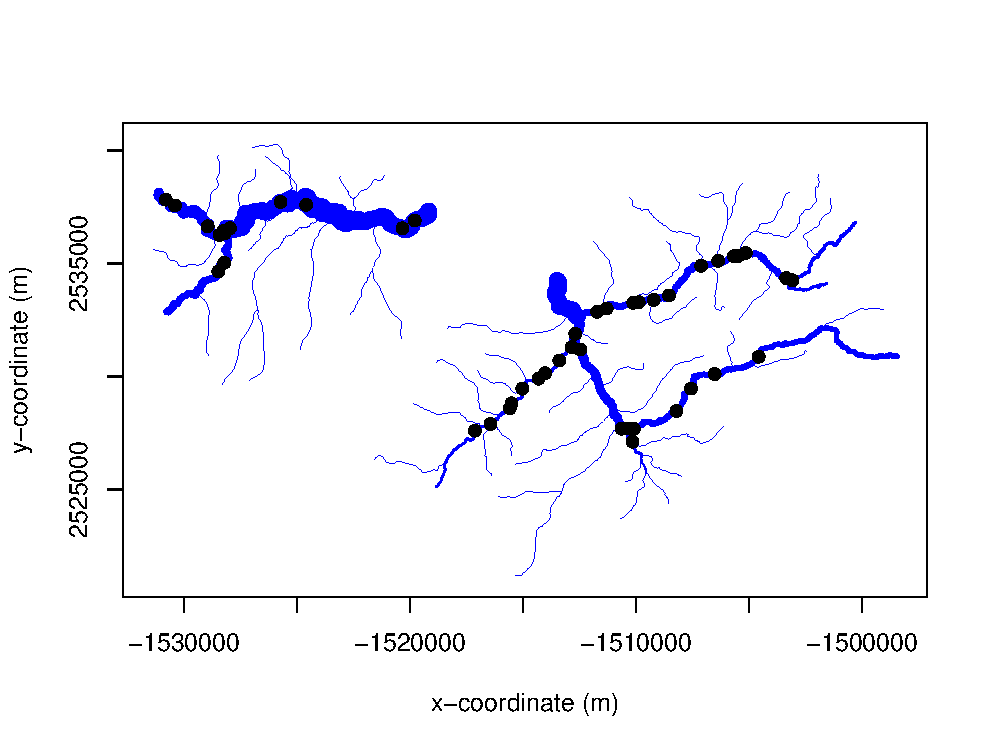
\includegraphics[keepaspectratio=true, width = 100mm]{Figures/jss984Fig-LoadData}
    \caption{A plot of the Middle Fork stream network. The locations
      of observed data are shown as black points. The
      blue lines indicate the river network and the thickness of these
      lines indicates the size of the river for each
      segment. \label{LoadData}}
  \end{center}
\end{figure}

Complex stream networks make it difficult to find the outlet, to tell
which stream segments lead to other segments, and which segments are
small or large. The line width in the plot can be made proportional to
a column in the \code{data} \code{data.frame} (Figure~\ref{SSNclass})
using the \code{lwdLineCol} and \code{lwdLineEx} arguments. The color
can also be set with \code{lineCol}.

Our example response variable, \code{Summer_mn}, is the average summer stream
temperature.  This response is plotted across the
stream network with observation locations colored by their value
(Figure~\ref{plotSpatialStreamNetwork}):

\begin{Schunk}
\begin{Sinput}
R> brks <- plot(mf04p, "Summer_mn", lwdLineCol = "afvArea",
+     lwdLineEx = 15, lineCol = "black", xlab =  "x-coordinate" ,
+     ylab =  "y-coordinate", asp=1 )
\end{Sinput}
\end{Schunk}

The arguments \code{color.palette}, \code{breaktype} and \code{brks}
control color scheme and break points. The plotting command returns a
matrix of break points that can be used later for consistency of color
meaning across multiple images.

\begin{figure}[htbp]
  \begin{center}
    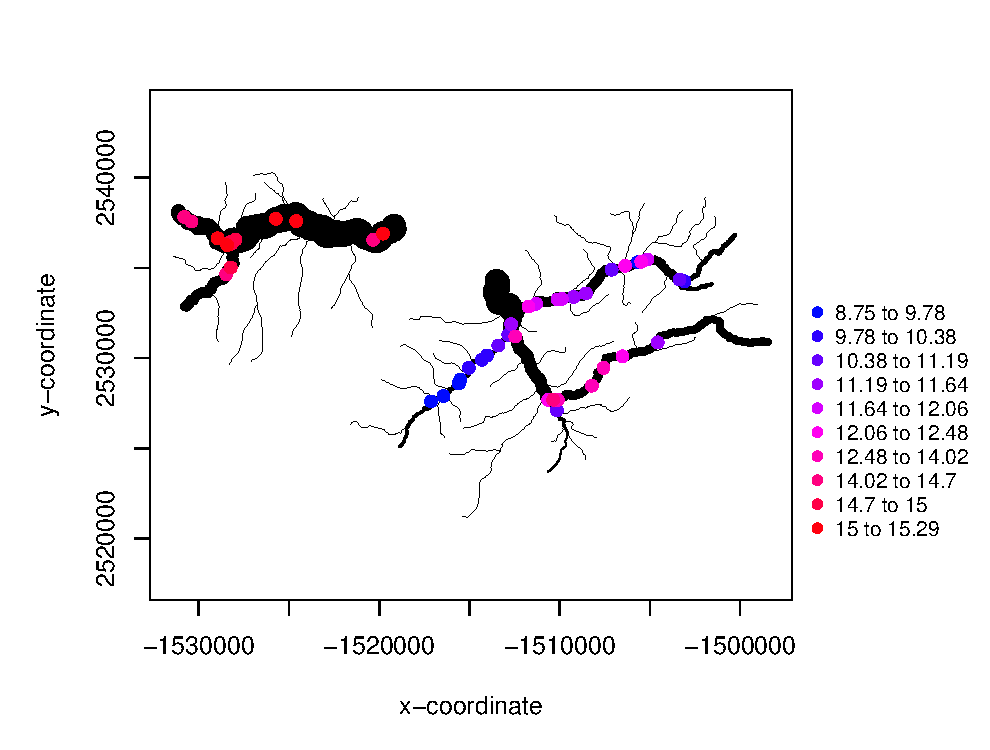
\includegraphics[keepaspectratio=true, width = 100mm]{Figures/jss984Fig-plotSpatialStreamNetwork}
    \caption{The generic plotting function of the
      \code{SpatialStreamNetwork} object for the Middle
      Fork data set. The observed values are
      represented by colored points and the stream network is shown in
      black, with the width of the lines proportional to the
      \code{afvArea} column.\label{plotSpatialStreamNetwork}}
  \end{center}
\end{figure}

Many users of spatial statistics are familiar with empirical semivariogram plots, which are used to understand how covariance changes with Euclidean distance. A new but similar graphic, called a Torgegram, is used for stream network data. The Torgegram computes average squared-differences like an empirical semivariogram, except that it is based on stream distance with the semivariance plotted separately for flow-connected and flow-unconnected pairs (see Figure~\ref{Torgegram}, where the size of the circles are proportional to the number of pairs for each binned distance class). Such figures were given in \citep{Ver:Pete:Theo:spat:2006, Ver:Pete:Move:2010}. The rationale behind a Torgegram is that autocorrelation may be evident only between flow-connected sites (e.g., for passive movement of chemical particles), while in other cases autocorrelation may be evident between flow-unconnected sites (e.g., for fish abundance because fish can move up-stream). Moreover, Section~\ref{TheoryModels} showed models that are more natural for autocorrelation among flow-connected sites only (Subsection~\ref{tailup}), those that also allow autocorrelation among flow-unconnected sites (Subsection~\ref{taildown}), and variance component approaches that combine them, along with models based on Euclidean distance (Subsection~\ref{sec:SpatialLinearMixedModels}).  The Torgegram is a visual tool for evaluating autocorrelation separately for flow-connected and flow-unconnected sites, and can help inform the selection of candidate models for fitting.  Further examples and discussion of the Torgegram are given in \citet{Pete:Ver:Isaa:stre:2013}.

Figure~\ref{Torgegram} is a plot of the Torgegram for the mean summer stream temperature:

\begin{Schunk}
\begin{Sinput}
R> mf04.Torg <- Torgegram(mf04p, "Summer_mn", nlag = 20, maxlag = 50000)
R> plot(mf04.Torg)
\end{Sinput}
\end{Schunk}

\begin{figure}[htbp]
  \begin{center}
    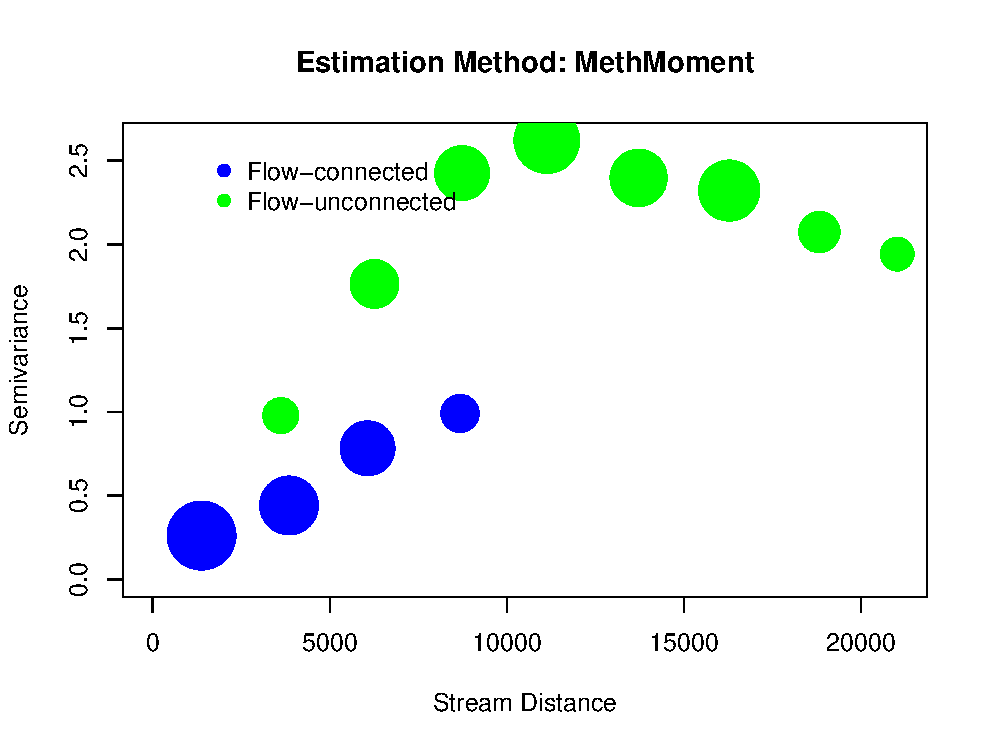
\includegraphics[keepaspectratio=true, width = 100mm]{Figures/jss984Fig-Torgegram}
    \caption{Torgegram of the mean summer temperature for the Middle
      Fork data set.\label{Torgegram}}
  \end{center}
\end{figure}

Close inspection of Figure~\ref{plotSpatialStreamNetwork} shows that neighboring locations on the stream network have very similar temperature values. Figure~\ref{Torgegram} shows that flow-connected sites have higher autocorrelation (lower semivariance) than flow-unconnected sites for the same distance when distances are short; however, both show high autocorrelation at short lags. Note that, for a stream network, there are longer in-stream distances when going from a head water to an outlet, and then back to a headwater (two flow-unconnected sites) than between a headwater and an outlet (two flow-connected sites).  The availability of longer flow-unconnected distances is shown in Figure~\ref{plotSpatialStreamNetwork}, where there are no flow-connected distances beyond 30000 m.  In Figure~\ref{plotSpatialStreamNetwork}, the semivariances increase to around 6 for flow-unconnected sites, and then start decreasing.  Flow-unconnected distances of near 50000 are from headwater to outlet to headwater, and the Torgegram shows more similarity for these sites than those separated by 30000 m.  This suggests including a covariate such as elevation, or simply distance upstream. This makes sense for temperature which will be colder at the higher elevations of the headwaters.  In summary, the Torgegram in Figure~\ref{Torgegram} suggests inclusion of elevation or distance upstream as a covariate in the linear model to account for an upstream trend in temperature, and based on the behavior of the Torgegram near the origin, both a tail-up and tail-down model will be necessary to capture the range of autocorrelation \citep{Ver:Pete:Move:2010}.  Later, the Torgegram will be used on residuals for model diagnostics.

% -------------------Model Fitting

\subsection{Model fitting}

The \code{glmssn} function fits a spatial linear model (Equation~\ref{eq:spLinearModel}) to a \code{SpatialStreamNetwork} object with a covariance structure shown in Equation~\ref{eq:covStructure}.  The ML or REML equations we optimized using the Nelder-Mead algorithm \citep{Neld:Mead:simp:1965} in the \code{optim} function. Covariance matrices are inverted numerically, which means that the computing time for $n$ observations increases proportionally to $n^3$, and is performed for each iteration of the ML or REML estimation method. This limits the size of data sets that can be fit by the \code{glmssn} function, and for most computing systems today we suggest sample sizes of less than 1000 observations.

An example of the \code{glmssn} function uses \code{Summer_mn} (mean
summer stream temperature) as a response variable from in the Middle
Fork data set. We include the covariates elevation and slope and
various spatial covariance components. The response and fixed effects
are specified using the \code{formula} argument, similar to \code{lm}
and \code{glm}. The input data set is specified with the \code{data}
argument, which must be a \code{SpatialStreamNetwork} object. The
\code{CorModels} argument is a list of correlation models. These
models should be of different types; i.e., at most one tail-up model,
one tail-down model, and one Euclidean distance model. The
\code{addfunccol} argument is the name of an additive function column,
which is required if a tail-up correlation model is included in
\code{CorModels}. More details can be found using
\code{help(glmssn)}. A non-spatial model is fitted:

% fit a basic model to look at likely covariates, variance components
% and diagnostics
\begin{Schunk}
\begin{Sinput}
R> mf04.glmssn0 <- glmssn(Summer_mn ~ ELEV_DEM + SLOPE, mf04p,
+     CorModels = NULL, use.nugget = TRUE)
R> summary(mf04.glmssn0)
\end{Sinput}
\begin{Soutput}
Call:
glmssn(formula = Summer_mn ~ ELEV_DEM + SLOPE, ssn.object = mf04p, 
    CorModels = NULL, use.nugget = TRUE)

Residuals:
    Min      1Q  Median      3Q     Max 
-2.3835 -1.1704  0.6205  0.9088  2.1930 

Coefficients:
              Estimate Std. Error t value Pr(>|t|)    
(Intercept)  62.839372  10.654190   5.898  < 2e-16 ***
ELEV_DEM     -0.024955   0.005379  -4.639    3e-05 ***
SLOPE       -88.019985  31.991343  -2.751  0.00872 ** 
---
Signif. codes:  0 '***' 0.001 '**' 0.01 '*' 0.05 '.' 0.1 ' ' 1

Covariance Parameters:
 Covariance.Model Parameter Estimate
           Nugget   parsill     1.81

Residual standard error: 1.344093
Generalized R-squared: 0.5625148
\end{Soutput}
\end{Schunk}

which can be compared to:

\begin{Schunk}
\begin{Sinput}
R> summary(lm(Summer_mn ~ ELEV_DEM + SLOPE, getSSNdata.frame(mf04p)))
\end{Sinput}
\begin{Soutput}
Call:
lm(formula = Summer_mn ~ ELEV_DEM + SLOPE, data = getSSNdata.frame(mf04p))

Residuals:
    Min      1Q  Median      3Q     Max 
-2.3835 -1.1704  0.6205  0.9088  2.1930 

Coefficients:
              Estimate Std. Error t value Pr(>|t|)    
(Intercept)  62.839372  10.654207   5.898 5.57e-07 ***
ELEV_DEM     -0.024955   0.005379  -4.639 3.40e-05 ***
SLOPE       -88.019985  31.991395  -2.751  0.00872 ** 
---
Signif. codes:  0 '***' 0.001 '**' 0.01 '*' 0.05 '.' 0.1 ' ' 1

Residual standard error: 1.344 on 42 degrees of freedom
Multiple R-squared:  0.5625,	Adjusted R-squared:  0.5417 
F-statistic:    27 on 2 and 42 DF,  p-value: 2.886e-08
\end{Soutput}
\end{Schunk}

A spatial model, including a mixture of tail-up, tail-down, and Euclidean
covariance models is fitted:

\begin{Schunk}
\begin{Sinput}
R> mf04.glmssn1 <- glmssn(Summer_mn ~ ELEV_DEM + SLOPE, mf04p,
+     CorModels = c("Exponential.tailup", "Exponential.taildown",
+        "Exponential.Euclid"), addfunccol = "afvArea")
R> summary(mf04.glmssn1)
\end{Sinput}
\begin{Soutput}
Call:
glmssn(formula = Summer_mn ~ ELEV_DEM + SLOPE, ssn.object = mf04p, 
    CorModels = c("Exponential.tailup", "Exponential.taildown", 
        "Exponential.Euclid"), addfunccol = "afvArea")

Residuals:
    Min      1Q  Median      3Q     Max 
-3.1839 -1.8289 -0.4117  0.2991  1.3447 

Coefficients:
              Estimate Std. Error t value Pr(>|t|)    
(Intercept)  64.817126  10.793922   6.005   <2e-16 ***
ELEV_DEM     -0.025756   0.005405  -4.765    2e-05 ***
SLOPE       -27.325550  14.868674  -1.838   0.0732 .  
---
Signif. codes:  0 '***' 0.001 '**' 0.01 '*' 0.05 '.' 0.1 ' ' 1

Covariance Parameters:
     Covariance.Model Parameter     Estimate
   Exponential.tailup   parsill      1.49392
   Exponential.tailup     range 117789.73261
 Exponential.taildown   parsill      0.00675
 Exponential.taildown     range 117751.99113
   Exponential.Euclid   parsill      0.07162
   Exponential.Euclid     range  38068.34362
               Nugget   parsill      0.01818

Residual standard error: 1.261142
Generalized R-squared: 0.4579287
\end{Soutput}
\end{Schunk}

It appears that slope is no longer a significant covariate when
comparing fits of the independence model to that with spatial
covariance.  It is often true that autocorrelated models yield fewer
factors with significant departures from zero.

The variable \code{MaxOver20} is a binary variable indicating if a
stream temperature value was over 20$^0$ C.  Here is an example of
fitting a spatial generalized linear model
(Section~\ref{SpGenLinMixMod}) to the binary data by using the
\code{family = "binomial"} argument:

\begin{Schunk}
\begin{Sinput}
R> mf04.glmssnBin <- glmssn(MaxOver20 ~ ELEV_DEM + SLOPE, mf04p,
+    CorModels = c("Mariah.tailup", "Spherical.taildown"),
+    family = "binomial", addfunccol = "afvArea")
R> summary(mf04.glmssnBin)
\end{Sinput}
\begin{Soutput}
Call:
glmssn(formula = MaxOver20 ~ ELEV_DEM + SLOPE, ssn.object = mf04p, 
    family = "binomial", CorModels = c("Mariah.tailup", "Spherical.taildown"), 
    addfunccol = "afvArea")

Residuals:
   Min     1Q Median     3Q    Max 
-3.001 -1.287 -1.070  1.312 11.614 

Coefficients:
             Estimate Std. Error t value Pr(>|t|)  
(Intercept)  59.16088   31.72727   1.865   0.0692 .
ELEV_DEM     -0.02988    0.01607  -1.859   0.0701 .
SLOPE       -74.43428  117.48688  -0.634   0.5298  
---
Signif. codes:  0 '***' 0.001 '**' 0.01 '*' 0.05 '.' 0.1 ' ' 1

Covariance Parameters:
   Covariance.Model Parameter   Estimate
      Mariah.tailup   parsill    0.29556
      Mariah.tailup     range    0.00213
 Spherical.taildown   parsill    0.39666
 Spherical.taildown     range 9627.05141
             Nugget   parsill    0.29981

Residual standard error: 0.9960069
Generalized R-squared: 0.09534395
\end{Soutput}
\end{Schunk}

The variable \code{C16} represents the number of summer days when the
stream temperature was greater than 16$^o$ C.  Here is an example of
fitting a spatial generalized linear model
(Section~\ref{SpGenLinMixMod}) to these count data by using the
\code{family = "poisson"} argument:

\begin{Schunk}
\begin{Sinput}
R> mf04.glmssnPoi <- glmssn(C16 ~ ELEV_DEM + SLOPE, mf04p,
+    CorModels = c("LinearSill.tailup", "LinearSill.taildown"),
+    family = "poisson", addfunccol = "afvArea")
R> summary(mf04.glmssnPoi)
\end{Sinput}
\begin{Soutput}
Call:
glmssn(formula = C16 ~ ELEV_DEM + SLOPE, ssn.object = mf04p, 
    family = "poisson", CorModels = c("LinearSill.tailup", "LinearSill.taildown"), 
    addfunccol = "afvArea")

Residuals:
     Min       1Q   Median       3Q      Max 
-1.00000 -0.18684 -0.01077  0.29539  1.25389 

Coefficients:
              Estimate Std. Error t value Pr(>|t|)   
(Intercept)  20.288563   6.763316   3.000  0.00453 **
ELEV_DEM     -0.008512   0.003430  -2.482  0.01715 * 
SLOPE       -12.198263  12.545956  -0.972  0.33647   
---
Signif. codes:  0 '***' 0.001 '**' 0.01 '*' 0.05 '.' 0.1 ' ' 1

Covariance Parameters:
    Covariance.Model Parameter       Estimate
   LinearSill.tailup   parsill     6.71742619
   LinearSill.tailup     range 19572.57825779
 LinearSill.taildown   parsill     0.98255198
 LinearSill.taildown     range   216.29881981
              Nugget   parsill     0.00000203

Residual standard error: 2.774884
Generalized R-squared: 0.179287
\end{Soutput}
\end{Schunk}

As one might expect, more high-temperature days are associated with
lower elevations and lower slopes, although the slope covariate is not
very significant.

% -------------------Residuals and Diagnostics

\subsection{Residuals and diagnostics}

The \code{residuals} function computes a collection of residual
diagnostics, including raw, standardized and Studentized residuals, as
well as fitted values and spatial versions of leverage and Cook's D
\citep{Cook:Weis:resi:1982}. For all computations other than raw
residuals, residual diagnostics use a modification of the classical
formulas developed for independent data. Standard independence
formulas are used for the linear model $\by^* = \bX^*\bbeta +
\bepsilon^*$, where $\bepsilon^*$ are independent errors, after
fitting the covariance matrix $\bSigma$ and then ``creating''
independent data as $\by^*=\bSigma^{-1/2}\by$ with a modified design
matrix $\bX^*=\bSigma^{-1/2}\bX$, where $\bSigma$ was defined in
Equation~\ref{eq:covStructure}. The result of the \code{residuals}
function is an \code{influenceSSN} object, which is an exact copy of
the \code{glmssn} object, except that residual diagnostics are
appended as new columns to the \code{point.data} \code{data.frame}
containing the observed data. The default plotting method for an
\code{influenceSSN} object is a map with color-coded raw residuals:

\begin{Schunk}
\begin{Sinput}
R> mf04.resid1 <- residuals(mf04.glmssn1)
R> names( getSSNdata.frame(mf04.resid1) )
\end{Sinput}
\begin{Soutput}
 [1] "pid"              "STREAMNAME"       "HUC3"            
 [4] "HUC4"             "COMID"            "CUMDRAINAG"      
 [7] "AREAWTMAP"        "MAXELEVSMO"       "SLOPE"           
[10] "NCEASID_"         "ELEV_DEM"         "Deployment"      
[13] "SampleYear"       "NumberOfDa"       "OriginalID"      
[16] "Source"           "Summer_mn"        "MaxOver20"       
[19] "C16"              "C20"              "C24"             
[22] "FlowCMS"          "AirMEANc"         "AirMWMTc"        
[25] "NEAR_FID"         "NEAR_DIST"        "NEAR_X"          
[28] "NEAR_Y"           "NEAR_ANGLE"       "rid"             
[31] "ratio"            "afvArea"          "upDist"          
[34] "locID"            "netID"            "computed.afv"    
[37] "obsval"           "_fit_"            "_resid_"         
[40] "_resid.stand_"    "_resid.student_"  "_leverage_"      
[43] "_CooksD_"         "_resid.crossv_"   "_CrossValPred_"  
[46] "_CrossValStdErr_"
\end{Soutput}
\begin{Sinput}
R> plot(mf04.resid1)
\end{Sinput}
\end{Schunk}

\begin{figure}[htbp]
  \begin{center}
    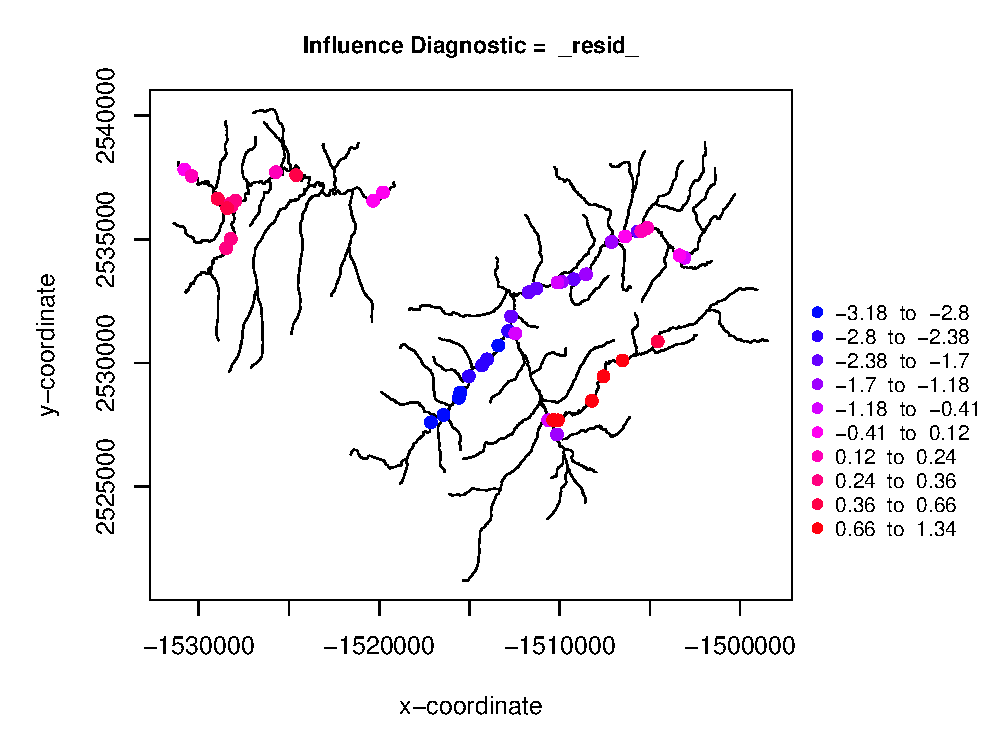
\includegraphics[keepaspectratio=true, width = 100mm]{Figures/jss984Fig-Model1}
    \caption{Plot of the raw residuals from fitting a model to the Middle Fork stream network. The legend on the right-hand side hints at the existence of residuals whose value are less than $-3$. \label{Model1}}
  \end{center}
\end{figure}

Columns added by the \code{residuals} function have names of the form
\code{_*_}. Maps of other diagnostics computed by \code{residuals} can
be plotted by using the \code{inflcol} argument.

Figure~\ref{Model1} indicates that there might be an outlier with a
residual less than $-3$. Histograms can be plotted of the raw
response variable and residuals.
(Figure~\ref{ResidHist}):

\begin{Schunk}
\begin{Sinput}
R> par(mfrow = c(1, 2))
R> hist(mf04.resid1)
R> hist(mf04p, "Summer_mn")
\end{Sinput}
\end{Schunk}

\begin{figure}[htbp]
  \begin{center}
    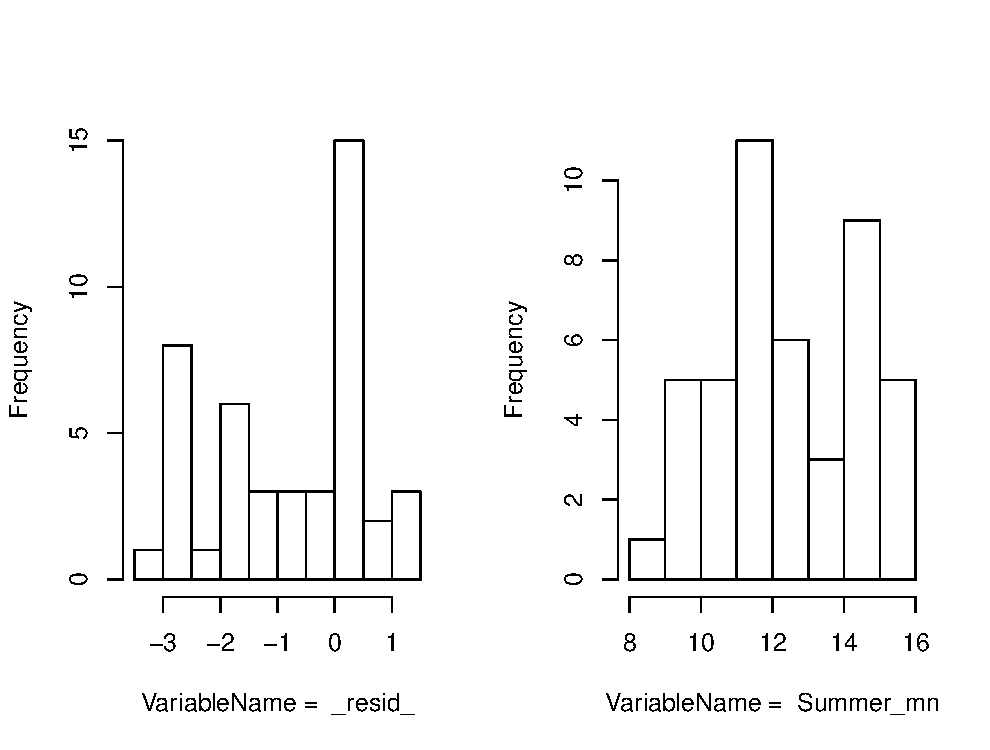
\includegraphics[keepaspectratio=true, width = 100mm]{Figures/jss984Fig-ResidHist}
    \caption{Histogram of the residuals (on the left) and a histogram of the average
      summer temperature values (on the right). \label{ResidHist}}
  \end{center}
\end{figure}

Let us treat the residual that is less than $-3$ as an outlier. We handle outliers by replacing their values with \code{NA}, which
will allow us to predict it later. First extract the {\tt data.frame}
of observed data and identify the record associated with the outlier,
insert an \code{NA} in the appropriate position for the response
variable, and then put the {\tt data.frame} back into the spatial
stream network object:

\begin{Schunk}
\begin{Sinput}
R> ObsDFr <- getSSNdata.frame(mf04.resid1)
R> ObsDF <- getSSNdata.frame(mf04p)
R> indOutlier <- ObsDFr["_resid_"] < -3
R> ObsDF[indOutlier, "Summer_mn"] <- NA
R> mf04c <- putSSNdata.frame(ObsDF, mf04p)
\end{Sinput}
\end{Schunk}

The new \code{SpatialStreamNetwork} object was renamed \code{mf04c}. Note that the outlier has been replaced in the \code{SpatialStreamNetwork} object, but not in the original data set in the \code{.ssn} directory. Having dealt with the outlier we refit the basic spatial model to the mean summer temperature, this time using ML rather than REML. We use ML because later we will use AIC for model selection, and REML cannot be used with AIC when fixed effects are changing \citep[][p. 75]{Verb:Mole:line:2000}.

\begin{Schunk}
\begin{Sinput}
R> mf04c.glmssn0 <- glmssn(Summer_mn ~ ELEV_DEM + SLOPE, mf04c,
+     CorModels = c("Exponential.tailup", "Exponential.taildown",
+     "Exponential.Euclid"), addfunccol = "afvArea", EstMeth = "ML")
R> summary(mf04c.glmssn0)
\end{Sinput}
\begin{Soutput}
Call:
glmssn(formula = Summer_mn ~ ELEV_DEM + SLOPE, ssn.object = mf04c, 
    CorModels = c("Exponential.tailup", "Exponential.taildown", 
        "Exponential.Euclid"), addfunccol = "afvArea", EstMeth = "ML")

Residuals:
    Min      1Q  Median      3Q     Max 
     NA -1.7829 -0.3289  0.3392      NA 

Coefficients:
             Estimate Std. Error t value Pr(>|t|)    
(Intercept)  64.29461   10.31964   6.230   <2e-16 ***
ELEV_DEM     -0.02551    0.00517  -4.934    1e-05 ***
SLOPE       -23.25010   15.03325  -1.547     0.13    
---
Signif. codes:  0 '***' 0.001 '**' 0.01 '*' 0.05 '.' 0.1 ' ' 1

Covariance Parameters:
     Covariance.Model Parameter    Estimate
   Exponential.tailup   parsill      1.3481
   Exponential.tailup     range 110976.5015
 Exponential.taildown   parsill      0.0485
 Exponential.taildown     range 117357.4743
   Exponential.Euclid   parsill      0.0180
   Exponential.Euclid     range  23667.8553
               Nugget   parsill      0.0177

Residual standard error: 1.196797
Generalized R-squared: 0.4416391
\end{Soutput}
\end{Schunk}

The partial sill associated with the exponential Euclidean model is quite low compared to the partial sills for the tail-up and tail-down models, as well as the nugget effect, and the fixed effect for \code{SLOPE} is also not significant, so they are dropped when refitting the model:

\begin{Schunk}
\begin{Sinput}
R> mf04c.glmssn1 <- glmssn(Summer_mn ~ ELEV_DEM, mf04c,
+     CorModels = c("Exponential.tailup", "Exponential.taildown"),
+     addfunccol = "afvArea", EstMeth = "ML")
R> summary(mf04c.glmssn1)
\end{Sinput}
\begin{Soutput}
Call:
glmssn(formula = Summer_mn ~ ELEV_DEM, ssn.object = mf04c, CorModels = c("Exponential.tailup", 
    "Exponential.taildown"), addfunccol = "afvArea", EstMeth = "ML")

Residuals:
    Min      1Q  Median      3Q     Max 
     NA -1.9503 -0.4230  0.0913      NA 

Coefficients:
             Estimate Std. Error t value Pr(>|t|)    
(Intercept) 69.876077  10.001403   6.987   <2e-16 ***
ELEV_DEM    -0.028273   0.005004  -5.650   <2e-16 ***
---
Signif. codes:  0 '***' 0.001 '**' 0.01 '*' 0.05 '.' 0.1 ' ' 1

Covariance Parameters:
     Covariance.Model Parameter      Estimate
   Exponential.tailup   parsill      1.815899
   Exponential.tailup     range 117791.352999
 Exponential.taildown   parsill      0.000795
 Exponential.taildown     range    226.290371
               Nugget   parsill      0.004710

Residual standard error: 1.349594
Generalized R-squared: 0.420658
\end{Soutput}
\end{Schunk}

Leave-one-out cross validation (LOOCV) provides a good diagnostic for
evaluating model performance. The function \code{CrossValidationSSN}
computes LOOCV predictions and standard errors for a fitted
\code{glmssn} object. The LOOCV predictions and standard errors are
included by default when using the \code{residual} function; column
names \code{_CrossValPred_} and \code{_CrossValStdErr_} are added to
the observed \code{point.data} \code{data.frame}, in addition to the
column \code{_resid.crossv_} which is the observed value subtracted
from \code{_CrossValPred_}. These variables can be mapped as
well. Figure~\ref{LOOCV} plots these LOOCV predictions and prediction
standard errors against the observed data.

\begin{Schunk}
\begin{Sinput}
R> cv.out <- CrossValidationSSN(mf04c.glmssn1)
R> par(mfrow = c(1, 2))
R> plot(mf04c.glmssn1$sampinfo$z,
+     cv.out[, "cv.pred"], pch = 19,
+     xlab = "Observed Data", ylab = "LOOCV Prediction")
R> abline(0, 1)
R> plot( na.omit( getSSNdata.frame(mf04c)[, "Summer_mn"]),
+     cv.out[, "cv.se"], pch = 19,
+     xlab = "Observed Data", ylab = "LOOCV Prediction SE")
\end{Sinput}
\end{Schunk}

\begin{figure}[htbp]
  \begin{center}
    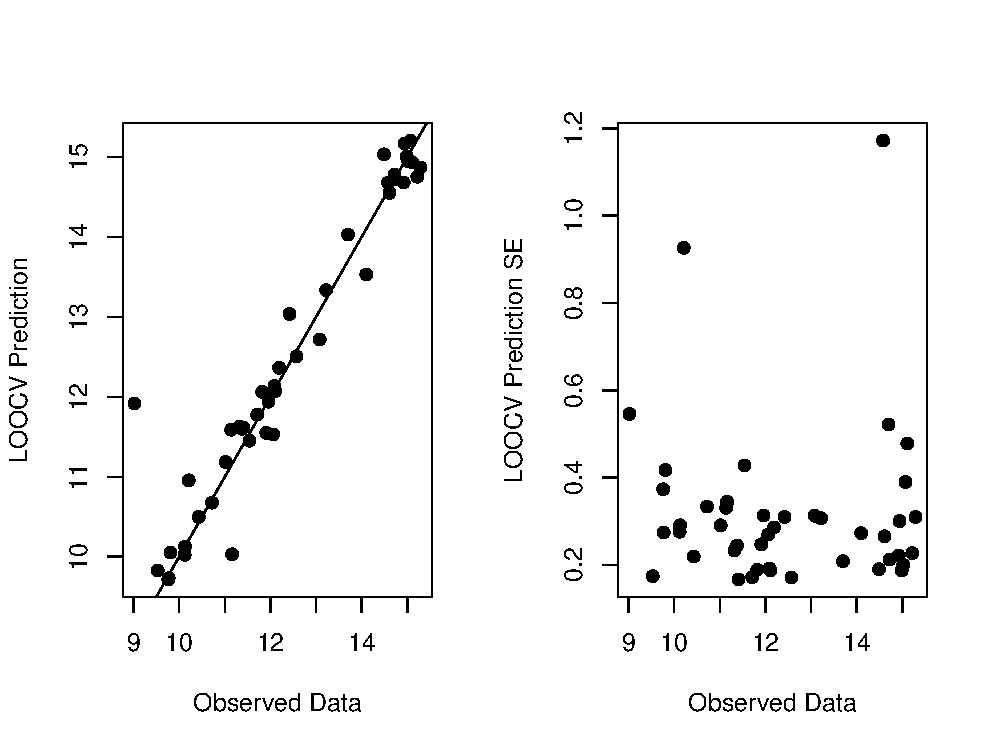
\includegraphics[keepaspectratio=true, width = 100mm]{Figures/jss984Fig-LOOCV}
    \caption{Leave-one-out cross validation predictions (on the left) and prediction
      standard errors (on the right) plotted against the observed response
      values.\label{LOOCV}}
  \end{center}
\end{figure}

The function \code{CrossValidationStatsSSN} both computes and
summarises the cross-validation statistics for a particular
\code{glmssn} object. Bias, root-mean-squared prediction error, and
confidence interval coverage are computed.

\begin{Schunk}
\begin{Sinput}
R> CrossValidationStatsSSN(mf04c.glmssn1)
\end{Sinput}
\begin{Soutput}
        bias   std.bias     RMSPE       RAV std.MSPE    cov.80
1 0.07892529 0.07445568 0.5467495 0.3680389 1.180716 0.7954545
     cov.90    cov.95
1 0.8409091 0.9090909
\end{Soutput}
\end{Schunk}

The \code{GR2} function computes a generalised R-squared for the
fitted \code{glmssn} object by computing the classical R-squared on
the $\by^* = \bX^*\bbeta + \bepsilon^*$ model.

The \code{varcomp} function takes the proportion of variation not
explained by the fixed effects (covariates) in \code{GR2}, and
apportions it by the partial sill of each spatial covariance
component.

\begin{Schunk}
\begin{Sinput}
R> GR2(mf04c.glmssn1)
\end{Sinput}
\begin{Soutput}
         [,1]
[1,] 0.420658
\end{Soutput}
\begin{Sinput}
R> varcomp(mf04c.glmssn1)
\end{Sinput}
\begin{Soutput}
               VarComp  Proportion
1    Covariates (R-sq) 0.420658045
2   Exponential.tailup 0.577590714
3 Exponential.taildown 0.000252963
4               Nugget 0.001498278
\end{Soutput}
\end{Schunk}

Here the fixed effects explains about 42\% of the variation in the
data, with the tail-up model contributing 57\% and very little from the tail-down and independent nugget
component.

% -------------------Model Selection

\subsection{Model selection}

Prior knowledge on the best model is rarely available, especially for
covariance structures, and so we often fit several and then compare
them in various ways. We fit \code{mf04c.glmssn0} and
\code{mf04c.glmssn1} using ML so that they could be compared using the
Akaike Information Criteria (AIC):

\begin{Schunk}
\begin{Sinput}
R> AIC(mf04c.glmssn0)
\end{Sinput}
\begin{Soutput}
[1] 100.2498
\end{Soutput}
\begin{Sinput}
R> AIC(mf04c.glmssn1)
\end{Sinput}
\begin{Soutput}
[1] 86.74482
\end{Soutput}
\end{Schunk}

It is clear that \code{SLOPE} is not a significant covariate.  Here,
we re-fit \code{mf04c.glmssn0} with REML (the default, so the
\code{EstMeth = "ML"} argument can be dropped), along with a few more
covariance structures:

\begin{Schunk}
\begin{Sinput}
R> mf04c.glmssn1 <- glmssn(Summer_mn ~ ELEV_DEM, mf04c,
+     CorModels = c("Exponential.tailup", "Exponential.taildown"),
+     addfunccol = "afvArea")
R> mf04c.glmssn2 <- glmssn(Summer_mn ~ ELEV_DEM,  mf04c,
+     CorModels = c("LinearSill.tailup", "Mariah.taildown"),
+     addfunccol = "afvArea")
R> mf04c.glmssn3 <- glmssn(Summer_mn ~ ELEV_DEM , mf04c,
+     CorModels =  c("Mariah.tailup", "LinearSill.taildown"),
+     addfunccol = "afvArea")
R> mf04c.glmssn4 <- glmssn(Summer_mn ~ ELEV_DEM, mf04c,
+     CorModels = c("Spherical.tailup", "Spherical.taildown"),
+     addfunccol = "afvArea")
R> mf04c.glmssn5 <- glmssn(Summer_mn ~ ELEV_DEM, mf04c,
+     CorModels = "Exponential.Euclid",
+     addfunccol = "afvArea")
\end{Sinput}
\end{Schunk}

Several different spatial models can be compared using the
\code{InfoCritCompare} command. This function extracts the AIC from
each model fit, evaluates the cross validation statistics for each
model and presents the results in table format:

\begin{Schunk}
\begin{Sinput}
R> options(digits = 4)
R> InfoCritCompare(list(mf04c.glmssn1, mf04c.glmssn2,
+     mf04c.glmssn3, mf04c.glmssn4, mf04c.glmssn5))
\end{Sinput}
\begin{Soutput}
               formula EstMethod
1 Summer_mn ~ ELEV_DEM      REML
2 Summer_mn ~ ELEV_DEM      REML
3 Summer_mn ~ ELEV_DEM      REML
4 Summer_mn ~ ELEV_DEM      REML
5 Summer_mn ~ ELEV_DEM      REML
                                 Variance_Components neg2LogL    AIC
1 Exponential.tailup + Exponential.taildown + Nugget    62.68  92.68
2       LinearSill.tailup + Mariah.taildown + Nugget    56.07  86.07
3       Mariah.tailup + LinearSill.taildown + Nugget    86.78 116.78
4     Spherical.tailup + Spherical.taildown + Nugget    57.42  87.42
5                        Exponential.Euclid + Nugget   126.54 144.54
        bias   std.bias  RMSPE    RAV std.MSPE cov.80 cov.90 cov.95
1  0.0703594  0.0661302 0.5300 0.3865   1.0445 0.7955 0.8864 0.9318
2  0.0759843  0.0680604 0.5042 0.3797   0.9103 0.7955 0.9091 0.9318
3  0.0570522  0.0569083 0.5053 0.5044   0.7416 0.8409 0.9318 0.9545
4  0.0786681  0.0713283 0.5262 0.3668   1.1189 0.7727 0.8182 0.9091
5 -0.0008186 -0.0004457 0.7863 0.8548   0.9261 0.8864 0.9091 0.9318
\end{Soutput}
\begin{Sinput}
R> options(digits = 7)
\end{Sinput}
\end{Schunk}

Note that AIC can be used with REML here because the fixed effects are
not changing among models. The comparisons show that all pure stream
network models do much better than one based on Euclidean
distance. Based on the low AIC value and the low root-mean-square
prediction error we decide on a final model that uses linear-with-sill tailup
and mariah taildown covariance structures.  Sample sizes are rather low, but
prediction intervals seem appropriate.  Here is summary of the final
fitted model:

\begin{Schunk}
\begin{Sinput}
R> summary(mf04c.glmssn2)
\end{Sinput}
\begin{Soutput}
Call:
glmssn(formula = Summer_mn ~ ELEV_DEM, ssn.object = mf04c, CorModels = c("LinearSill.tailup", 
    "Mariah.taildown"), addfunccol = "afvArea")

Residuals:
     Min       1Q   Median       3Q      Max 
      NA -2.06272 -0.55153 -0.01528       NA 

Coefficients:
             Estimate Std. Error t value Pr(>|t|)    
(Intercept) 69.500614   9.110772   7.628   <2e-16 ***
ELEV_DEM    -0.028026   0.004546  -6.166   <2e-16 ***
---
Signif. codes:  0 '***' 0.001 '**' 0.01 '*' 0.05 '.' 0.1 ' ' 1

Covariance Parameters:
  Covariance.Model Parameter     Estimate
 LinearSill.tailup   parsill      2.55170
 LinearSill.tailup     range 116389.88234
   Mariah.taildown   parsill      0.00145
   Mariah.taildown     range  54764.16600
            Nugget   parsill      0.02348

Residual standard error: 1.605188
Generalized R-squared: 0.5012196
\end{Soutput}
\end{Schunk}

In addition to outliers from a fitted model (i.e., global outliers),
outliers may exist with respect to predictions that do not appear as
large deviations from the fit.  A histogram of standardized LOOCV
prediction residuals can identify local prediction outliers
(Figure~\ref{Residuals}):

\begin{Schunk}
\begin{Sinput}
R> mf04c.resid2 <- residuals(mf04c.glmssn2)
R> mf04c.resid2.cv.std <-
+      getSSNdata.frame(mf04c.resid2)[, "_resid.crossv_"] /
+      getSSNdata.frame(mf04c.resid2)[, "_CrossValStdErr_"]
R> hist(mf04c.resid2.cv.std)
\end{Sinput}
\end{Schunk}

\begin{figure}[htbp]
  \begin{center}
    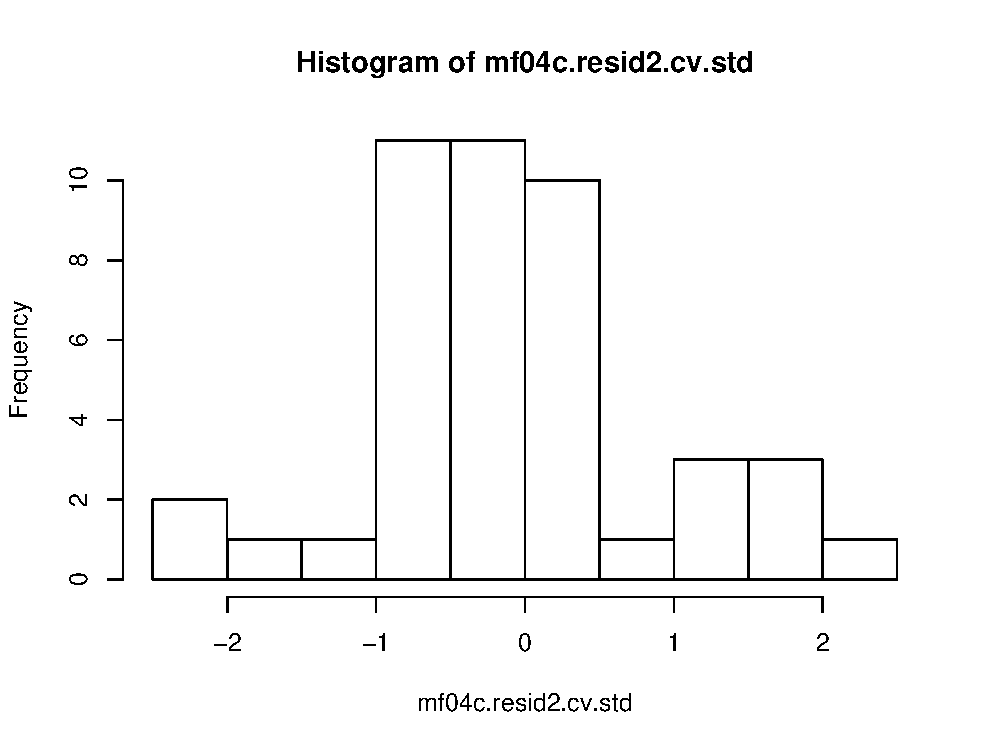
\includegraphics[keepaspectratio=true, width = 100mm]{Figures/jss984Fig-Residuals}
    \caption{Histogram of standardized cross-validation residuals for
      model \code{mf04c.glmssn2} of mean summer stream temperature for the Middle Fork
      stream network with \code{ELEV\_DEM} covariate and spherical tail-up, spherical tail-down and nugget covariance components.\label{Residuals}}
  \end{center}
\end{figure}

When fitting covariates, spatial autocorrelation is modeled on the
errors, so a Torgegram of the residuals helps visualize the spatial
pattern after fitting the fixed effects.  Note that this is imperfect
because the fitted model is not a simple function of distance; it is
complicated by weighting for tail-up models, and by asymmetry in
distances for tail-down models \citep[see][Figure
7]{Ver:Pete:Move:2010}. A Torgegram on the residuals of
\code{mf04c.glmssn2} is given in Figure~\ref{TorgRes}:

\begin{Schunk}
\begin{Sinput}
R> plot(Torgegram(mf04c.resid2, "_resid_", nlag = 8, maxlag = 25000))
\end{Sinput}
\end{Schunk}

\begin{figure}[htbp]
  \begin{center}
    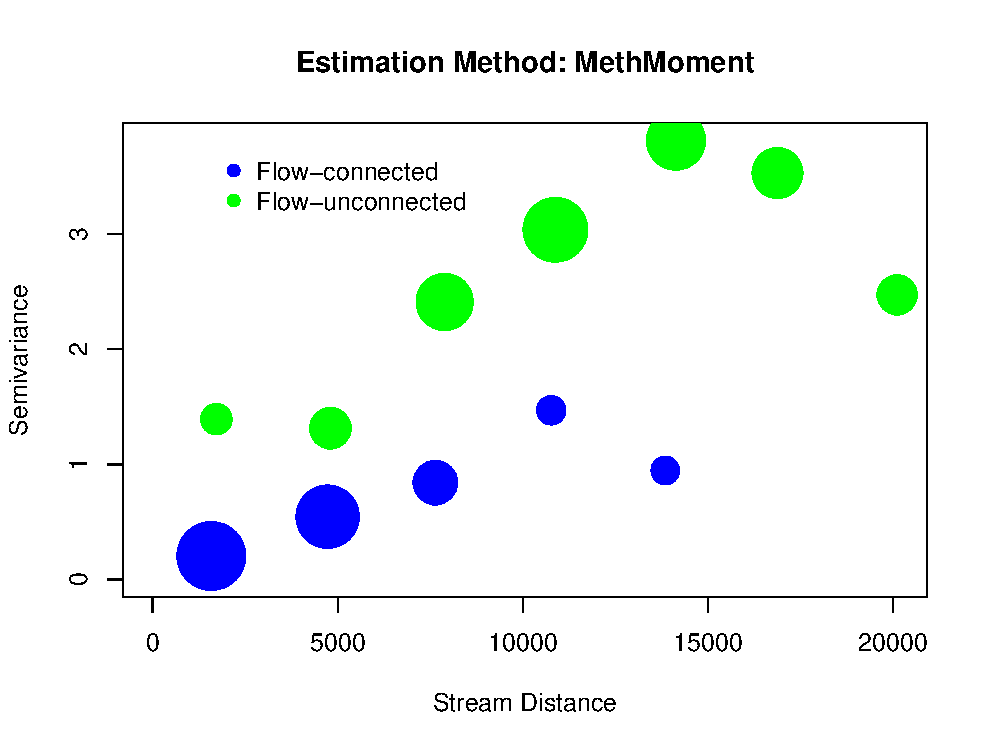
\includegraphics[keepaspectratio=true, width = 100mm]{Figures/jss984Fig-TorgRes}
    \caption{Torgegram of residuals for model \code{mf04c.glmssn2} of mean summer
      temperature in the Middle Fork stream network with \code{ELEV\_DEM} covariate and spherical tail-up, spherical tail-down and nugget covariance components.\label{TorgRes}}
  \end{center}
\end{figure}

Figure~\ref{TorgRes} shows apparent autocorrelation for both
flow-connected and flow-unconnected sites, although flow-unconnected sample sizes are small for short lags, supporting the decision to use both tail-up and tail-down models, even though the partial sill for tail-down model contributes little to the overall variability of the error.  The overall sill is modeled to be slightly greater than 2.5. 

% -------------------Prediction

\subsection{Prediction}

Two functions for prediction are included in the \code{SSN} package:
\code{predict} and \code{BlockPredict}, which are also known as
(universal) kriging and (universal) block kriging, respectively.

As a first example, we predict at point locations in the
\code{pred1km} data set (Figure~\ref{Preds1}). The size of the
prediction points indicates the prediction standard errors; larger
points have lower prediction standard errors, so if we are more
confident in a point it stands out more in the graphic. Previously
defined breakpoints are used here, so the colours in
Figure~\ref{Preds1} match those found earlier in
Figure~\ref{plotSpatialStreamNetwork}.

\begin{Schunk}
\begin{Sinput}
R> mf04c.pred1km <- predict(mf04c.glmssn4, "pred1km")
R> plot(mf04c.pred1km, SEcex.max = 1, SEcex.min = .5/3*2,
+       breaktype = "user", brks = brks)
\end{Sinput}
\end{Schunk}

\begin{figure}[htbp]
  \begin{center}
    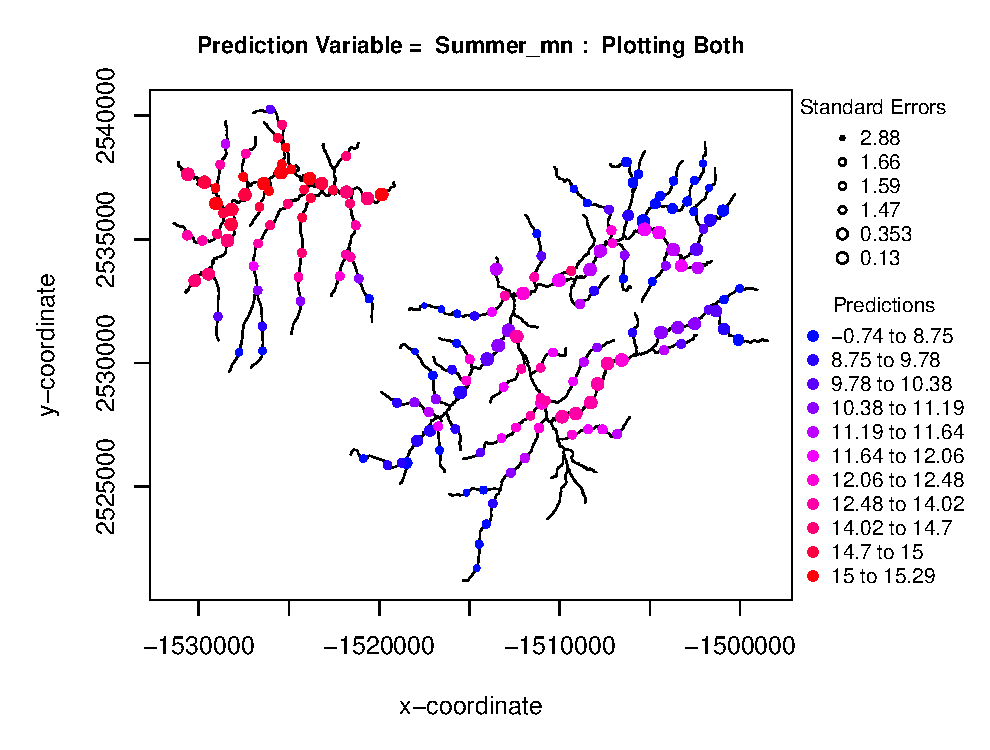
\includegraphics[keepaspectratio=true, width = 100mm]{Figures/jss984Fig-Preds1}
    \caption{Predictions of mean summer temperature values for the Middle Fork stream network. Predicted
      values are indicated by the color of the circles. The size of
      the circles is inversely related to the prediction standard
      error.}\label{Preds1}
  \end{center}
\end{figure}

The second prediction data set is made up of a dense set of points
along a single tributary, called Knapp Creek, of the Middle Fork
river. We predict all points using the \code{predict} function. In
Figure~\ref{Preds2} we first plotted the observed values with large
open circles in the vicinity of the Knapp tributary, with values
color-coded. We then added the Knapp predictions, which use the same
break points as the first plot. Note that text is automatically added
for the lowest and highest predicted values:

\begin{Schunk}
\begin{Sinput}
R> plot(mf04c, "Summer_mn", pch = 1, cex = 3,
+     xlab = "x-coordinate", ylab = "y-coordinate",
+     xlim = c(-1511000,-1500000), ylim = c(2525000,2535000))
R> mf04c.glmssn4.Knapp <- predict(mf04c.glmssn4, "Knapp")
R> plot(mf04c.glmssn4.Knapp, "Summer_mn", add = TRUE,
+     xlim = c(-1511000,-1500000), ylim = c(2525000,2535000))
\end{Sinput}
\end{Schunk}

\begin{figure}[htbp]
  \begin{center}
    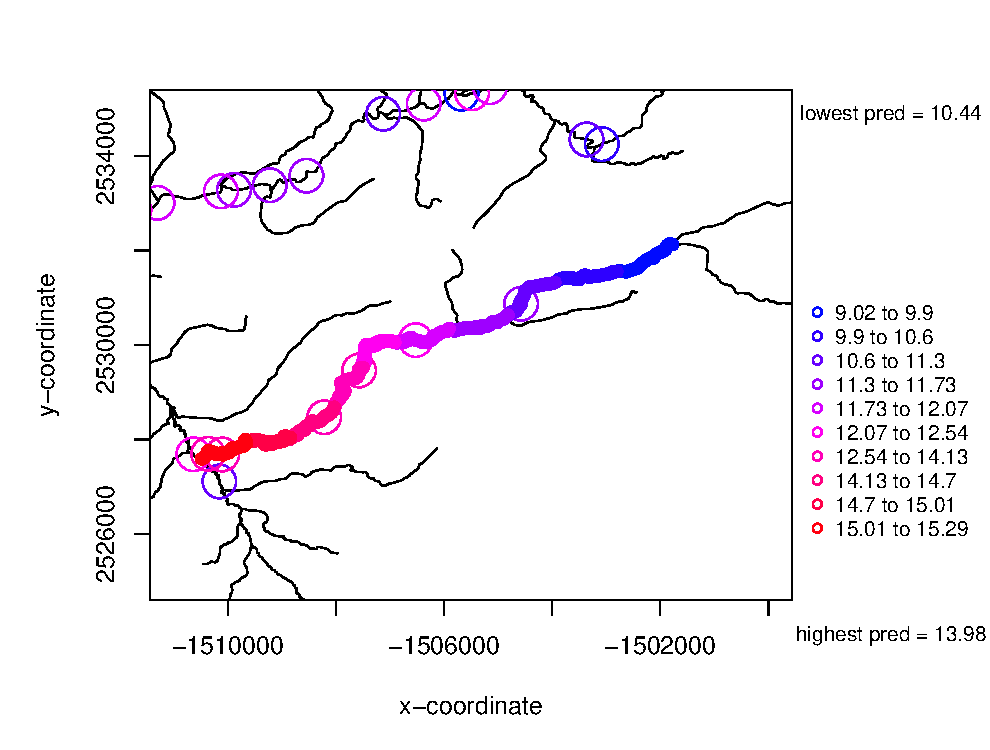
\includegraphics[keepaspectratio=true, width = 100mm]{Figures/jss984Fig-Preds2}
    \caption{Predictions of mean summer stream temperature values
      along Knapp Creek. Predicted values are filled circles
      and observed data are large open circles. Color breaks are based
      on the full data set, but the map is zoomed-in to Knapp Creek. \label{Preds2}}
  \end{center}
\end{figure}
By using matching break points for observed data and predicted data,
we can see that predictions seem reasonable given the observed data.

The prediction sites are on a dense evenly-spaced grid because they
are used to approximate the integrals involved with block prediction:
\begin{Schunk}
\begin{Sinput}
R> mf04c.glmssn4.BPKnapp <- BlockPredict(mf04c.glmssn4, "Knapp")
R> mf04c.glmssn4.BPKnapp
\end{Sinput}
\begin{Soutput}
  BlockPredEst BlockPredSE
1      12.3197  0.09913953
\end{Soutput}
\end{Schunk}
We can repeat this for another set of spatially dense locations on the
Cape Horn tributary of the Middle Fork river:
\begin{Schunk}
\begin{Sinput}
R> mf04c.glmssn4.BPCapeHorn <- BlockPredict(mf04c.glmssn4, "CapeHorn")
R> mf04c.glmssn4.BPCapeHorn
\end{Sinput}
\begin{Soutput}
  BlockPredEst BlockPredSE
1     10.02122   0.0477452
\end{Soutput}
\end{Schunk}
The predicted block average values, along with the standard errors of
block prediction, allow comparison between these two reaches.

Finally, recall that we replaced an outlier value with \code{NA} when
creating \code{mf04c} from \code{mf04}. When fitting a model with
\code{glmssn}, records with \code{NA} response values are used to
create a new prediction data set, called \code{_MissingObs_}, in the
fitted \code{glmssn} object. \code{_MissingObs_} is like any other
prediction data set and can be used to predict the \code{NA}s. We
compare the original outlier value with this prediction:

\begin{Schunk}
\begin{Sinput}
R> mf04c.missingobs <- predict(mf04c.glmssn4, "_MissingObs_")
R> getPreds(mf04c.missingobs, pred.type = "pred")
\end{Sinput}
\begin{Soutput}
     pid Summer_mn Summer_mnPredSE
[1,]  29  9.668828       0.7183271
\end{Soutput}
\begin{Sinput}
R> with(getSSNdata.frame(mf04p), Summer_mn[pid==29])
\end{Sinput}
\begin{Soutput}
[1] 8.75
\end{Soutput}
\end{Schunk}

Notice that the original value is within the 95\% prediction
interval at that point, so it probably was not an outlier.

% ------------------------------------------------------------------------------
%
%                   SIMULATING STREAM NETWORK DATA
%
% ------------------------------------------------------------------------------

\section{Simulating stream network data}\label{Simulation}

The \pkg{SSN} package can be used to simulate stream network data,
which involves two steps: 1) creating a \code{SpatialStreamNetwork}
object, and 2) simulating an autocorrelated response variable for a
\code{SpatialStreamNetwork} object. These functions can be used for
testing methods, comparing sampling methods, etc., and were used
extensively for testing functions when developing the \pkg{SSN}
package.

% -------------------Creating an SSN Object

\subsection[Creating a SpatialStreamNetwork object]{Creating a \code{SpatialStreamNetwork} object}

The \pkg{SSN} package provides the function \code{createSSN} for
constructing \code{SpatialStreamNetwork} objects based on randomly
generated networks, with randomly generated observation and prediction
points. There are two approaches to generating a random
network. First, notice that stream networks are tree structures that
are a special type of graph, so random graph functions in \proglang{R}
can be used to generate such a structure. However, these functions are
not spatially explicit so every vertex requires a position in the
plane for a graph-drawing algorithm, which is an additional step. The
second approach is to write more customised code that generates a
network and assigns positions to vertices while generating the
network.

The first approach has several downsides; few of the methods for
generating random graphs can be used to generate tree structures, and
existing graph-drawing algorithms tend to give a highly regular
network structure or a structure with self-intersections, which we do not consider in our models of river systems. The second approach has none of these
downsides but may be slower computationally. Both approaches are
implemented in the \pkg{SSN} package.

The \code{createSSN} function has the form
\begin{Schunk}
\begin{Sinput}
R> createSSN(n, obsDesign, predDesign = noPoints, path,
+     importToR = FALSE, treeFunction = igraphKamadaKawai)
\end{Sinput}
\end{Schunk}

The argument \code{n} is a integer vector where the length of the
vector is the number of networks and each integer is the number of
stream segments per network. The \code{path} argument gives the full
path name where the \code{.ssn} directory associated with the new
\code{SpatialStreamNetwork} object will be stored, and
\code{importToR} determines whether the created object will be loaded
and returned directly from this function. The arguments
\code{obsDesign} and \code{predDesign} specify sampling design
functions that allow the user to control how the observation and
prediction points are generated. The simplest input is a single point
for \code{obsDesign} and no prediction points \code{predDesign =
noPoints}, which generates no points.

The argument \code{treeFunction} controls how the random tree
structure is generated. There are currently two possible values, with
the default of \code{igraphKamadaKawai} taking the first approach
above and using random graph methods. We use the \pkg{igraph} package
and the Kamada-Kawai graph drawing algorithm from the same package
\citep{Csar:Nepu:2006}. The second possible value is
\code{iterativeTreeLayout} which can produce more realistic networks
and is guaranteed not to create any self-intersections.  An example of
the types of networks generated by this layout is given in
Figure~\ref{SimIterative}.

\begin{Schunk}
\begin{Sinput}
R> set.seed(12)
R> iterative.ssn <- createSSN(n = c(30, 10),
+     obsDesign = binomialDesign(c(10,10)),
+     importToR = TRUE, path = "./SimIterative.ssn",
+     treeFunction = iterativeTreeLayout)
R> plot(iterative.ssn, lwdLineCol = "addfunccol", lwdLineEx = 8,
+     lineCol = "blue", cex = 2, xlab = "x-coordinate",
+     ylab = "y-coordinate", pch = 1)
\end{Sinput}
\end{Schunk}

\begin{figure}[htbp]
  \begin{center}
    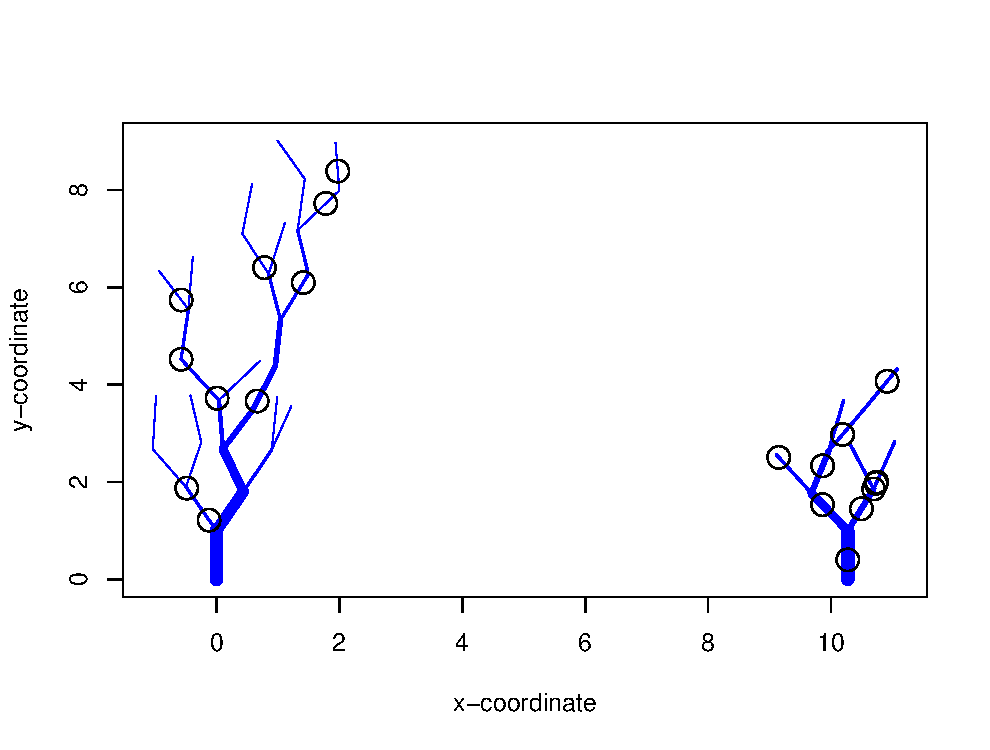
\includegraphics[keepaspectratio=true, width = 100mm]{Figures/jss984Fig-SimIterative}
    \caption{The network is generated using \code{iterativeTreeLayout}
      and the points are generated using the \code{hardCoreDesign}
      function. \label{SimIterative}}
  \end{center}
\end{figure}
%%

A number of design functions are provided, including
\begin{itemize}
\item \code{poissonDesign(lambda)}
\item \code{hardCoreDesign(n, inhibition_region)}
\item \code{systematicDesign(spacing)}
\item \code{binomialDesign(n)}.
\end{itemize}
Input \code{lambda} is a numeric vector specifying (on a per-network
basis) the rate of occurance of points for the Poisson process, while
for the binomial design \code{n} specifies the number of points to be
generated from a uniform distribution across each network. The
\code{systematicDesign} function is more complicated, and is intended
to generate a set of regular points, especially useful for block
prediction.  Note that in our implementation for networks this means
every point is a constant distance from the next most downstream
point, so points just upstream of a junction may be very close to each
other, and on visual inspection the points may not appear to be
equally spaced.  This constant spacing is specified by the input
\code{inhibition_region}.  The \code{hardCoreDesign} generates
\code{n} randomly distributed points on each network, and then removes
points until the remainder are all at least \code{inhibition_region}
distant from each other.  Examples of \code{systematicDesign} and
\code{hardCoreDesign} are given in Figures~\ref{SimSSN1} and
\ref{SimHardcore} respectively.

\begin{Schunk}
\begin{Sinput}
R> set.seed(101)
R> raw.ssn <- createSSN(n = c(10, 10, 10),
+     obsDesign = binomialDesign(c(40, 40, 40)),
+     predDesign = systematicDesign(c(0.2, 0.4, 0.8)), importToR = TRUE,
+     path = "./raw.ssn")
R> plot(raw.ssn, lwdLineCol = "addfunccol", lwdLineEx = 8,
+     lineCol = "blue", cex = 2, xlab = "x-coordinate",
+     ylab = "y-coordinate", pch = 1)
R> plot(raw.ssn, PredPointsID = "preds", add = TRUE, cex = .5, pch = 19,
+     col = "green")
\end{Sinput}
\end{Schunk}

\begin{Schunk}
\begin{Sinput}
R> set.seed(13)
R> hardcore.ssn <- createSSN(n = c(10, 10),
+     obsDesign = hardCoreDesign(c(200, 200), c(0.2, 0.4)),
+     importToR = TRUE, path = "./SimHardcore.ssn")
R> plot(hardcore.ssn, lwdLineCol = "addfunccol", lwdLineEx = 8,
+     lineCol = "blue", cex = 2, xlab = "x-coordinate",
+     ylab = "y-coordinate", pch = 1)
R> plot(hardcore.ssn, PredPointsID = NULL, add = TRUE, cex = .5,
+     pch = 19, col = "green")
\end{Sinput}
\end{Schunk}

%% Now include the figure
\begin{figure}[htb]
  \begin{center}
    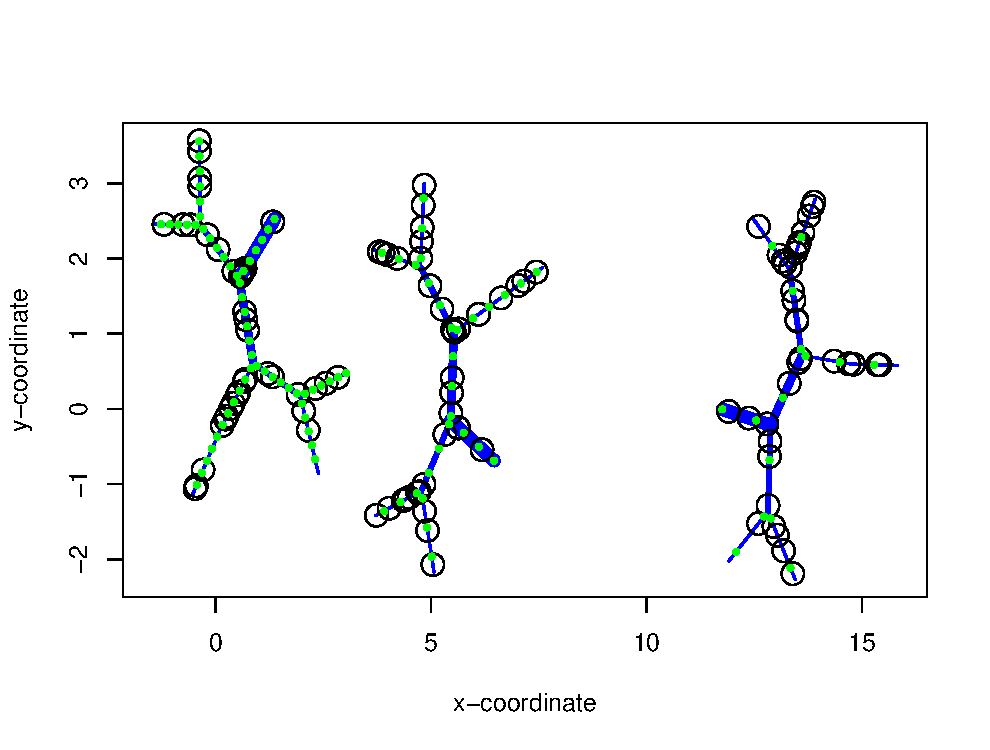
\includegraphics[keepaspectratio=true, width = 100mm]{Figures/jss984Fig-SimSSN1}
    \caption{Three simulated stream networks. The blue lines get
      thinner farther up-stream. The open black circles are observed
      locations, and the smaller solid green points are prediction
      locations generated by \code{systematicDesign}. \label{SimSSN1}}
  \end{center}
\end{figure}

\begin{figure}[htbp]
  \begin{center}
    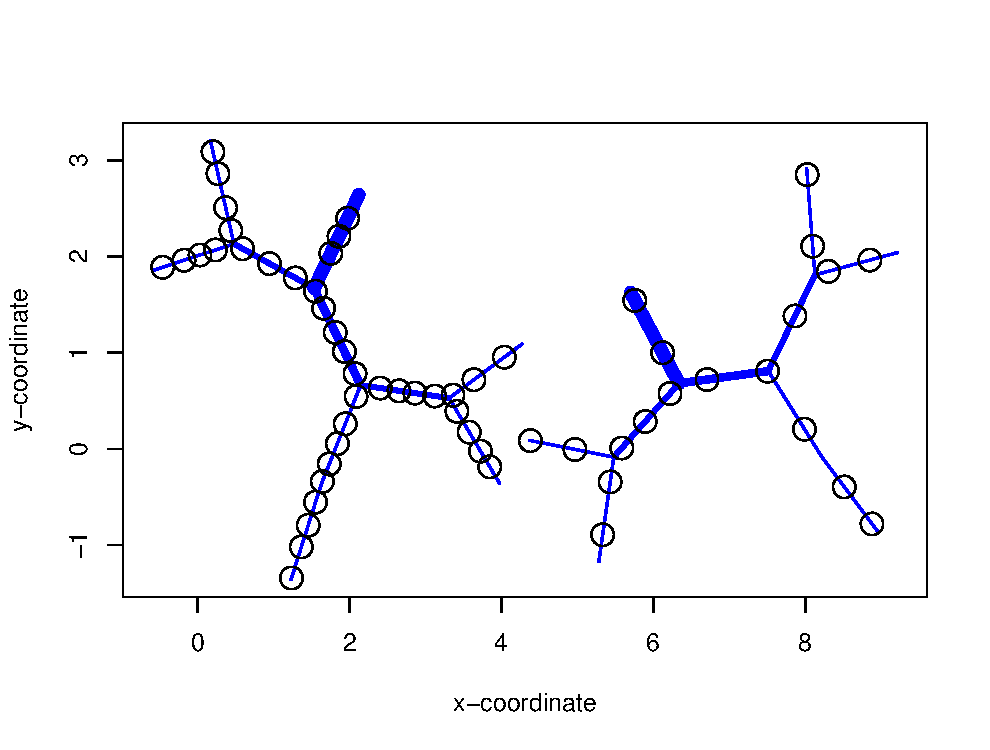
\includegraphics[keepaspectratio=true, width = 100mm]{Figures/jss984Fig-SimHardcore}
    \caption{Points generated by \code{hardCoreDesign}, with varying
      inhibition regions. The blue lines get thinner farther up-stream. The open black circles are simulated
      locations, which have a more regular pattern than the spatially random locations shown by the open circles in Figure~\ref{SimSSN1}. \label{SimHardcore}}
  \end{center}
\end{figure}

While there are only four design functions built into the package, it
is possible for the user to construct their own sampling design
functions, and then generate location data using the \code{createSSN}
function.


% -------------------Simulating the SSN object

\subsection[Simulating data on the SpatialStreamNetwork object]{Simulating data on the \code{SpatialStreamNetwork} object}

After creating a \code{SpatialStreamNetwork} object (e.g.,
Figure~\ref{SimSSN1}), we may want to simulate on both observed and
prediction locations.  This functionality is useful for developing and
testing new statistical methods and code, as well as for model
diagnostics for real data, such as examining realized patterns of
hypothetical or fitted models.  First, the distance matrices among all
points is created:

\begin{Schunk}
\begin{Sinput}
R> createDistMat(raw.ssn, "preds", o.write=TRUE, amongpred = TRUE)
\end{Sinput}
\end{Schunk}

Note the \code{amongpred} argument.  For simulation, we need a
covariance matrix (computed from the distance matrix) among prediction
locations, which is typically not needed for spatial modeling of
observed locations or predicting at prediction locations.  This matrix
can be quite large so some care should be taken about its size,
otherwise \proglang{R} will run out of memory or predictions will take
a long time to compute.  The first step is to extract the
\code{point.data} \code{data.frame}s for the observed and prediction
locations from the \code{SpatialStreamNetwork} object:

\begin{Schunk}
\begin{Sinput}
R> rawDFobs <- getSSNdata.frame(raw.ssn, "Obs")
R> rawDFpred <- getSSNdata.frame(raw.ssn, "preds")
\end{Sinput}
\end{Schunk}

Continuous covariates are created in each \code{data.frame}:

\begin{Schunk}
\begin{Sinput}
R> rawDFobs[,"X1"] <- rnorm(length(rawDFobs[,1]))
R> rawDFpred[,"X1"] <- rnorm(length(rawDFpred[,1]))
R> rawDFobs[,"X2"] <- rnorm(length(rawDFobs[,1]))
R> rawDFpred[,"X2"] <- rnorm(length(rawDFpred[,1]))
\end{Sinput}
\end{Schunk}

Categorical covariates can also be created:

\begin{Schunk}
\begin{Sinput}
R> rawDFobs[,"F1"] <- as.factor(sample.int(4,length(rawDFobs[,1]),
+     replace = TRUE))
R> rawDFpred[,"F1"] <- as.factor(sample.int(4,length(rawDFpred[,1]),
+     replace = TRUE))
\end{Sinput}
\end{Schunk}

Random effects are created just like a categorical covariates; in this
example one is created with three levels and another with four levels:

\begin{Schunk}
\begin{Sinput}
R> rawDFobs[,"RE1"] <- as.factor(sample(1:3,length(rawDFobs[,1]),
+     replace = TRUE))
R> rawDFobs[,"RE2"] <- as.factor(sample(1:4,length(rawDFobs[,1]),
+     replace = TRUE))
R> rawDFpred[,"RE1"] <- as.factor(sample(1:3,length(rawDFpred[,1]),
+     replace = TRUE))
R> rawDFpred[,"RE2"] <- as.factor(sample(1:4,length(rawDFpred[,1]),
+     replace = TRUE))
\end{Sinput}
\end{Schunk}

The list of column names for the \code{data.frame}s now includes the
new covariates:
\begin{Schunk}
\begin{Sinput}
R> names(rawDFobs)
\end{Sinput}
\begin{Soutput}
 [1] "locID"      "upDist"     "pid"        "netID"      "rid"       
 [6] "ratio"      "shreve"     "addfunccol" "NEAR_X"     "NEAR_Y"    
[11] "X1"         "X2"         "F1"         "RE1"        "RE2"       
\end{Soutput}
\begin{Sinput}
R> names(rawDFpred)
\end{Sinput}
\begin{Soutput}
 [1] "locID"      "upDist"     "pid"        "netID"      "rid"       
 [6] "ratio"      "shreve"     "addfunccol" "NEAR_X"     "NEAR_Y"    
[11] "X1"         "X2"         "F1"         "RE1"        "RE2"       
\end{Soutput}
\end{Schunk}

For prediction, it is important to make sure that the observed and
prediction \code{data.frame}s have the same set of columns for any
specification of random or fixed effects.

Note that the creation of the \code{SpatialStreamNetwork} object
included Shreve's stream order, and the additive function value is
based on Shreve's and is contained in the \code{addfunccol} column for
each location, which is required for tail-up models as described in
Section~\ref{tailup}.

To simulate data on the SpatialStreamNetwork object, use the
\code{SimulateOnSSN} function:

\begin{Schunk}
\begin{Sinput}
R> set.seed(102)
R> sim.out <- SimulateOnSSN(raw.ssn, ObsSimDF = rawDFobs,
+     PredSimDF = rawDFpred, PredID = "preds",
+     formula = ~ X1 + X2 + F1, coefficients = c(10,1,0,-2,0,2),
+     CorModels = c("LinearSill.tailup", "Mariah.taildown",
+     "Exponential.Euclid", "RE1", "RE2"), use.nugget = TRUE,
+     CorParms = c(3, 10, 2, 10, 1, 5, 1, .5, .1),
+     addfunccol = "addfunccol")
\end{Sinput}
\end{Schunk}

The \code{ObsSimDF} argument replaces the observed \code{point.data}
\code{data.frame} in \code{raw.ssn} with \code{rawDFobs}.  For that
reason, it is best to use \code{getSSNdata.frame} to extract the
original observed \code{point.data} \code{data.frame} in
\code{raw.ssn} to make sure it complies with the object structure, and
then modify its covariates if desired. Likewise, the \code{PredSimDF}
argument replaces the prediction \code{point.data} \code{data.frame}
in \code{raw.ssn} with \code{rawDFpred}. The function
\code{SimulateOnSSN} simulates and stores data in a new column,
\code{"Sim{\textunderscore}Values"} in both \code{point.data}
\code{data.frames}.

The one-sided formula specifies how the fixed effects are computed,
which works just like an \proglang{R} formula in other functions.  A
design matrix $\bX$ is created from the \code{formula} input, and the
mean value is computed as $\bmu = \bX\bbeta$. Hence, coefficients
$\bbeta$ must be specified using the \code{coefficients} argument.
Some understanding of how \proglang{R} creates design matrices is
necessary in order to apply the coefficients properly.  In our
example, the first column of the design matrix $\bX$ will be all ones
for an overall intercept, as that is the default in a formula
specification.  The next two columns will contain the covariate values
of {\tt X1} and {\tt X2}.  Because there is an overall intercept, the
model is over-parameterized for the categorical covariate and so the
first level of {\tt F1} is dropped and 0-1 dummy variables are created
for the other three levels. The column names of the design matrix can
be examined
\begin{Schunk}
\begin{Sinput}
R> with(rawDFobs, colnames(model.matrix( ~ X1 + X2 + F1)))
\end{Sinput}
\begin{Soutput}
[1] "(Intercept)" "X1"          "X2"          "F12"        
[5] "F13"         "F14"        
\end{Soutput}
\end{Schunk}
or the whole matrix can be examined by removing the \code{colnames}
function. The \code{coefficients} argument creates the $\bbeta$ in the
order given in the argument and multiplies it with the design matrix
created by the \code{formula} argument.

Likewise, the rules for covariance matrix construction require careful
consideration.  Regardless of the order of \code{CorModel}
specification, the subset of parameters will be in the order of
$\btheta=(\sigma^2_u, \alpha_u,\sigma^2_d, \alpha_d, \sigma^2_e,
\alpha_e, \sigma^2_1, \ldots, \sigma^2_p, \sigma^2_0)$, so the
\code{CorParms} argument should be used to match this order.  Note
that there can only be a single tail-up model, a single tail-down
model, and a single Euclidean distance model.  Any factor variable can
be used to create random effects, and the inclusion of the
\code{nugget = TRUE} argument includes $\sigma^2_0$ in the covariance
model.

The output of the {\tt SimulateOnSSN} function is a list with three
objects.  Two of those objects simply verify that the
\code{coefficients} and \code{CorParms} were used as intended.  For
our example:

\begin{Schunk}
\begin{Sinput}
R> sim.out$FixedEffects
\end{Sinput}
\begin{Soutput}
       Xnames Coefficient
1 (Intercept)          10
2          X1           1
3          X2           0
4         F12          -2
5         F13           0
6         F14           2
\end{Soutput}
\begin{Sinput}
R> sim.out$CorParms
\end{Sinput}
\begin{Soutput}
            CorModel    type Parameter
1  LinearSill.tailup parsill       3.0
2  LinearSill.tailup   range      10.0
3    Mariah.taildown parsill       2.0
4    Mariah.taildown   range      10.0
5 Exponential.Euclid parsill       1.0
6 Exponential.Euclid   range       5.0
7                RE1 parsill       1.0
8                RE2 parsill       0.5
9             nugget parsill       0.1
\end{Soutput}
\end{Schunk}

The simulated SpatialStreamNetwork object can be extracted:
\begin{Schunk}
\begin{Sinput}
R> sim.ssn <- sim.out$ssn.object
\end{Sinput}
\end{Schunk}

and plotting yields Figure~\ref{SimSSN2}:
%% this plot returns a value as well as produces a plot, we use
%% results=hide to suppress the returned value.
\begin{Schunk}
\begin{Sinput}
R> plot(sim.ssn, "Sim_Values",
+     xlab = "x-coordinate", ylab = "y-coordinate",
+     cex = 1.5)
\end{Sinput}
\end{Schunk}

which shows simulated values at the locations created in
Figure~\ref{SimSSN1}. Note that response values were also simulated at prediction locations in Figure~\ref{SimSSN1}, but are not shown.
\begin{figure}[h]
  \begin{center}
    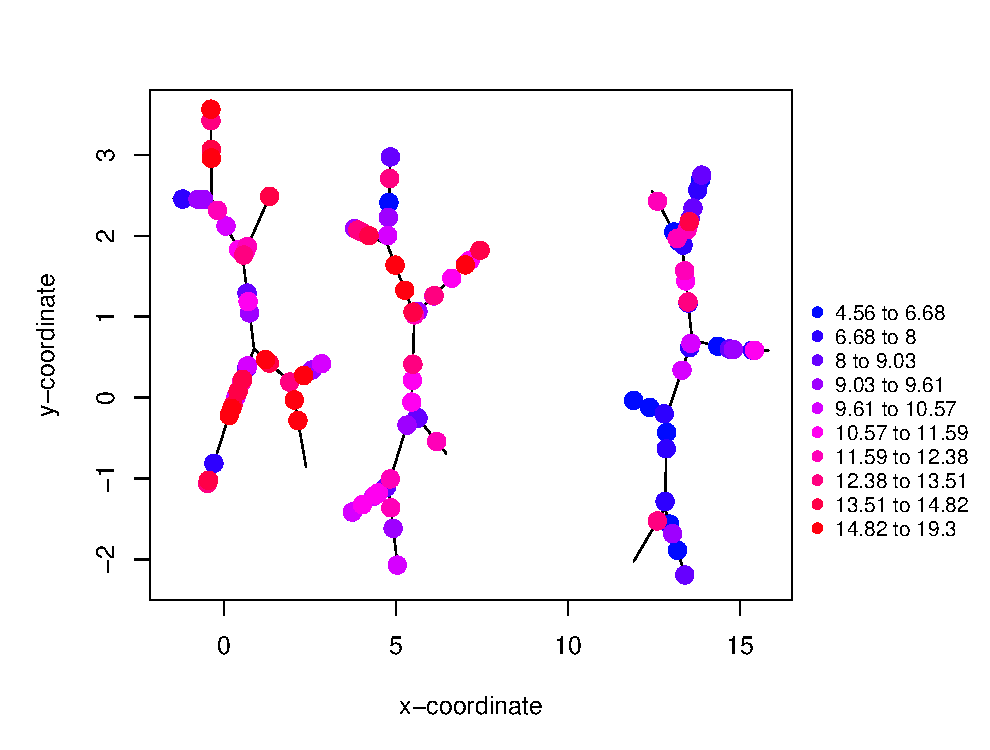
\includegraphics[keepaspectratio=true, width = 100mm]{Figures/jss984Fig-SimSSN2}
    \caption{Values for the response variable were simulated at the simulated observed locations shown in Figure~\ref{SimSSN1}. The simulated data are colored by their values, showing an autocorrelated response. \label{SimSSN2}}
  \end{center}
\end{figure}

To test the function, extract the observed and predicted
\code{point.data} \code{data frame}s, which now contain simulated
values:
\begin{Schunk}
\begin{Sinput}
R> simDFobs <- getSSNdata.frame(sim.ssn, "Obs")
R> simDFpred <- getSSNdata.frame(sim.ssn, "preds")
\end{Sinput}
\end{Schunk}

To test prediction, we stored the simulated prediction values and
replaced them with \code{NA}s:
\begin{Schunk}
\begin{Sinput}
R> simpreds <- simDFpred[,"Sim_Values"]
R> simDFpred[,"Sim_Values"] <- NA
R> sim.ssn <- putSSNdata.frame(simDFpred, sim.ssn, "preds")
\end{Sinput}
\end{Schunk}

We fit a model to the simulated data to see how well the simulation
parameters are estimated:
\begin{Schunk}
\begin{Sinput}
R> glmssn.out <- glmssn(Sim_Values ~ X1 + X2 + F1, sim.ssn,
+     CorModels = c("LinearSill.tailup", "Mariah.taildown",
+     "Exponential.Euclid", "RE1", "RE2"),
+     addfunccol = "addfunccol")
\end{Sinput}
\end{Schunk}

yielding output:
\begin{Schunk}
\begin{Sinput}
R> summary(glmssn.out)
\end{Sinput}
\begin{Soutput}
Call:
glmssn(formula = Sim_Values ~ X1 + X2 + F1, ssn.object = sim.ssn, 
    CorModels = c("LinearSill.tailup", "Mariah.taildown", "Exponential.Euclid", 
        "RE1", "RE2"), addfunccol = "addfunccol")

Residuals:
    Min      1Q  Median      3Q     Max 
-6.8831 -1.5712 -0.3135  1.4124  7.5558 

Coefficients:
            Estimate Std. Error t value Pr(>|t|)    
(Intercept) 11.15167    2.44131   4.568    1e-05 ***
X1           0.86409    0.09849   8.773   <2e-16 ***
X2           0.02523    0.08464   0.298    0.766    
F11          0.00000         NA      NA       NA    
F12         -2.50504    0.27903  -8.978   <2e-16 ***
F13         -0.18864    0.27122  -0.696    0.488    
F14          1.66940    0.25403   6.572   <2e-16 ***
---
Signif. codes:  0 '***' 0.001 '**' 0.01 '*' 0.05 '.' 0.1 ' ' 1

Covariance Parameters:
   Covariance.Model Parameter Estimate
  LinearSill.tailup   parsill  5.48953
  LinearSill.tailup     range  6.08873
    Mariah.taildown   parsill  1.39656
    Mariah.taildown     range  2.49147
 Exponential.Euclid   parsill  7.02589
 Exponential.Euclid     range 66.91703
                RE1   parsill  1.23216
                RE2   parsill  0.01551
             Nugget   parsill  0.00579

Residual standard error: 3.894284
Generalized R-squared: 0.8165259
\end{Soutput}
\end{Schunk}

If we compare the fixed-effects estimates to the coefficients
specified in the \code{SimulateOnSSN} function, it appears that they
are estimated quite well. The covariance parameters are not estimated
as well. This is not surprising because there are quite a few of them,
and even though they may individually be far from their simulation
values, the actual covariance matrix based on them can be quite close
to the original covariance matrix, especially near the origin, which
is most critical \citep{Stei:asym:1988}.  Finally, the predictions
from the fitted model are compared to the actual values that were
simulated:
\begin{Schunk}
\begin{Sinput}
R> glmssn.pred <- predict(glmssn.out,"preds")
R> predDF <- getSSNdata.frame(glmssn.pred, "preds")
R> plot(simpreds, predDF[,"Sim_Values"], xlab = "True",
+     ylab = "Predicted", pch = 19)
\end{Sinput}
\end{Schunk}

\begin{figure}
  \begin{center}
    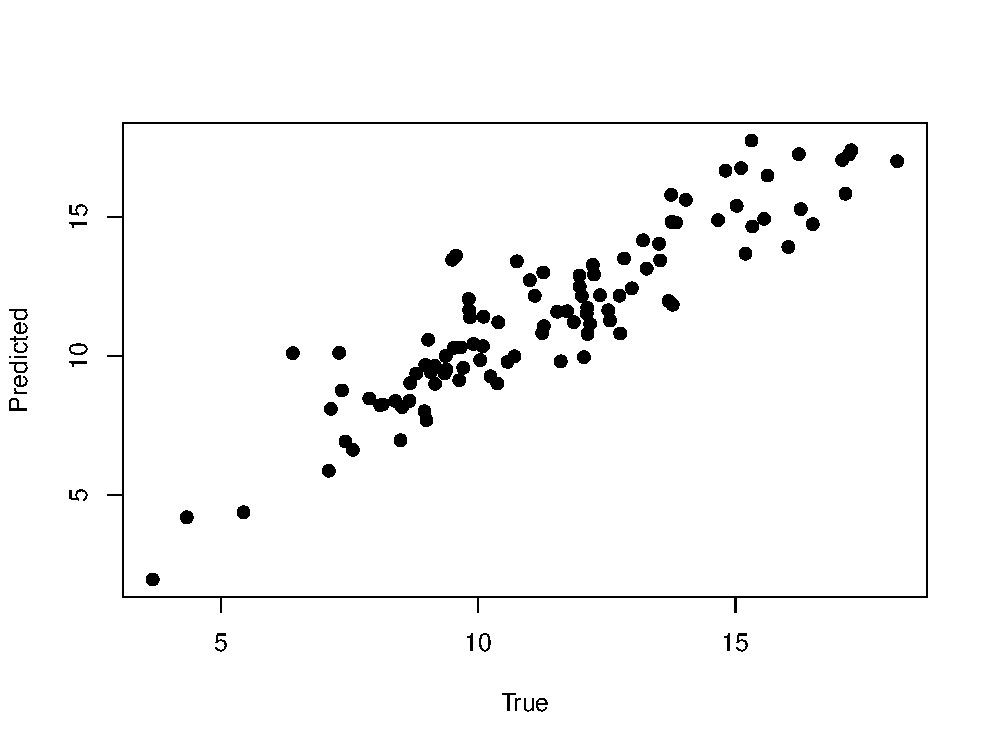
\includegraphics[keepaspectratio=true, width = 100mm]{Figures/jss984Fig-SimTvP}
    \caption{A comparison of true simulated data and predictions at
      locations after true values were removed.\label{SimTrueVsPred}}
  \end{center}
\end{figure}
Figure~\ref{SimTrueVsPred} shows excellent prediction accuracy, which
relied on both covariates and autocorrelation.


% ------------------------------------------------------------------------------
%
%                          FUTURE DEVELOPMENT
%
% ------------------------------------------------------------------------------

\section{Discussion and future development}\label{FutureDev}

In the Introduction, we noted that the \pkg{Rtop} package can also be used for prediction on stream networks. The model, called topological kriging, was developed in \citet{Skoi:Merz:Blos:top:2006}.  The basic idea is to create random variables as block means of a spatial random field (with point support) for all basin area above a point on a stream.  This will create nested blocks for locations that share flow and create strong correlation among them, while locations that do not share flow will be correlated by proximity in the blocks.  Because correlation is based on both nesting and proximity, \citet{Laah:Skoi:Blos:comp:2012} argue that topological kriging should be better than the methods given in \pkg{SSN}.  However, \citet{Ver:Pete:Move:2010} and the \pkg{SSN} as demonstrated here advance the idea that the best use of the models is to combine the tail-up, tail-down, and Euclidean distance models in a variance component approach. In fact, this approach allows for pure stream-distance models, to pure Euclidean distance models, and combinations thereof, so it should be more flexible than \pkg{Rtop}.  Also, by using likelihood methods, \pkg{SSN} allows fitting linear models with valid inference on covariate effects, in addition to spatial prediction.  Regardless of any conceptual argument, the availability of both \pkg{SSN} and \pkg{Rtop} should allow for interesting comparisons between the methods and hopefully spur development in both areas.

We plan to refine the \pkg{SSN} package, making function calls more flexible, which will give users more control over how a plot looks or even to define their own functions for parameter estimation.  Currently, we have only implemented the Poisson and binomial families, but plan to extend this to many more families similar to other generalized linear model fitting functions in \proglang{R}.  Similarly, data transformation such as Box-Cox \citep{Box:Cox:anal:1964} with lognormal and trans-gaussian kriging \citep[][p. 135-138]{Cres:stat:1993} will be implemented, and newer methods such as nonparametric transformations \citep{Grib:Kriv:new:2012} will be investigated. We also plan to extend the \code{createSSN} function so that observed and prediction locations may be generated on existing stream network shapefiles. Another major goal is to implement more efficient model-fitting algorithms for data sets with large numbers of observation sites (e.g., > 2000), such as those collected using in-stream sensor networks \citep{Port:Hans:Lin:stay:2012}. The estimation of model parameters currently requires the iterative inversion of a matrix with dimensions given by the number of observation sites, which can be computationally intensive when the number of those sites is larger than 2000. \proglang{R} can be compiled with support for more advanced linear algebra packages such as the Intel Math Kernel Library (MKL) \url{http://software.intel.com/en-us/articles/intel-mkl/}, and this results in substantial speed improvements.  However, new model-fitting algorithms will be needed before a geostatistical model can be fit to data sets on the order of 20000 or more observations. Currently, large numbers of prediction sites (>50000) are possible because prediction of individual sites only requires a single inverse of a matrix with dimensions given by the number of observation sites. 


% ------------------------------------------------------------------------------
%
%                  SECTION ACKNOWLEDGMENTS
%
% ------------------------------------------------------------------------------

\section{Acknowledgments}

Support for this work was provided by the United States (US) Forest
Service, the US Geological Survey, and the Oregon State Office of the
Bureau of Land Management. Some of this work was conducted as part of
the working group entitled ``Spatial Statistics for Streams,'' supported by the National Center for Ecological Analysis
and Synthesis, a Center funded by NSF (Grant \#EF-0553768), the
University of California, Santa Barbara, and the State of
California. This project also received financial support from the
CSIRO Water for a Healthy Country Flagship, and the NOAA's National
Marine Fisheries Service to the Alaska Fisheries Science Center. We
also thank Devin Johnson and Jeff Laake for constructive reviews of a
previous version of this manuscript. Reference to trade names does not
imply endorsement by the National Marine Fisheries Service, NOAA. The
findings and conclusions in the paper are those of the authors and do
not necessarily represent the views of the National Marine Fisheries
Service.


% ------------------------------------------------------------------------------
%
%                       REFERENCES
%
% ------------------------------------------------------------------------------

\bibliography{jss984}


\end{document}
